\section{Introduction}
\label{sec:priointro}
Priority is an important concept in modeling workflows. For instance, modeling compensation and error handling requires a mechanism to express priority of some flow alternatives over others. In the context of Reo, priority can be utilized as a mechanism to impose preferences on the otherwise non-deterministic choices.

%when several transitions are possible, the network chooses one of them in a non-deterministic fashion. However, in some cases for instance when this non-deterministic choice is between a critical flow and a normal flow, we would like to impose our preference on the non-deterministic choice.  
%???There is ongoing work on an existing automata based formal semantics of Reo to handle priority, but our practical needs for dealing with large models of realistic business processes currently complicates direct use of automata-based semantic models.
%
% Figure \ref{fig:prioritymerger} depicts. The behavior of \emph{priority merger} is defined in terms of coloring semantics.
%
%\begin{figure}[!h]
%\centering
%    \scriptsize
%        \tikz{
%          \node[state] (q) {};
%          \node[state, right of=q, node distance=5cm] (p) {m};
%          \path[transition] (q) edge [loop above] node {$\{\},\textit{true}$} (q); 
%          \path[transition] (q) edge [bend left] node {$\{a, b, e\},\hat{a}=\hat{b} \wedge \hat{b}=\hat{e} \wedge \hat{m}'=\hat{e}$}  (p);     
%          \path[transition] (q) edge [bend right] node {$\{c,d,e\},\hat{d}=\hat{e} \wedge \hat{m}'=\hat{e}$}  (p);
%          \path[transition] (p) edge [loop above] node {$\{\},\textit{true}$} (p); 
%          \path[transition] (p) edge  node {$\{f\}, \hat{m}=\hat{f}$}  (q);                            
%        }
%   \label{fig:prioritymerger}
%   \caption{Priority Merger}
%\end{figure}
%
%Addressing priority as a distinct concept from context-sensitivity in Reo networks requires explicit notion. 
%Arbab et al. ~\cite{priority} introduce several channels to incorporate in the open-ended set or Reo channels that provide an expressive framework to allow imposing, propagating and blocking the priority and its propagation. 

Arbab et al. in ~\cite{priority} introduce a compositional approach to model priority and a priority-aware formal semantics for Reo, named Constraint Automata with Priority (CAP), which is an extension of constraint automata.

This approach, which distinguishes between where priority is originated from and where it must be applied i.e. non-deterministic choices, consists of the following elements:

\begin{itemize}
 \item A primitive to impose priority that is \emph{prioritySync},
 \item A mechanism to propagate priority from the location it is imposed through the network,
 \item A mechanism to block the propagation of priority in desired places using one of the following primitives:  
 \begin{itemize}
 \item \emph{BlockSourceSync}, which stops propagation of priority coming from its source end toward its sink;
 \item \emph{BlockSinkSync}, which blocks propagation of priority from its sink end toward its source; 
 \item \emph{BlockSync} that stops propagation of priority on both ends.
 \end{itemize}
\item Means to affect the otherwise non-deterministic choices by priority.
\label{item:prioreq}
\end{itemize}

CAP is an expressive formalism for supporting priority in Reo. However, its operations to manipulate CAPs are computationally expensive, if they are implemented in a straight-forward fashion. %Moreover, similar to CA, CAP does not formalize existence of I/O requests on nodes, which is referred to as context. Context is needed to explicitly express conditions in which a transition of higher priority is not feasible due to lack of request; and therefore, a lower priority transition occurs.   

The practical needs for dealing with large models of realistic business processes currently complicates direct use of automata-based semantic models. 
%Therefore, we extend our constraint-based framework with priority encoding constraints. Our approach %constraint framework to obtain priority-aware semantics of Reo connectors
% benefits from efficient optimized off-the-shelf constraint solvers. Since the framework already includes connector coloring semantics, by reflecting context information in constraints that describe behavior of a Reo connector, we can explicitly express aforementioned conditions.  %This explicit information is useful for instance in analyzing and  executing Reo connectors. 
  %
In this chapter, we extend our constraint-based framework presented in Chapter \ref{chapterCASM} to support priority in Reo.
 %Our approach consists of the following elements:
 %
 %\begin{itemize}
 %	\item We use the \emph{PrioritySync} primitive to impose priority, 
 %	\item We present a model to propagate the priority through the network that is similar to connector coloring semantics,
 %	\item We use \emph{BlockSourceSync}, \emph{BlockSinkSync}, and \emph{BlockSync} to block the propagation of priority in desired places,
%	\item We extend our constraint-based framework to incorporate the propagated priority information.
 %\end{itemize} 
 The rest of this chapter is organized as follows: In Section~\ref{sec:example}, we introduce priority flow in Reo along with a constraint-based semantics for it. In Section~\ref{sec:extension}, we extend our approach to support numeric priorities. In Section~\ref{casestudy}, we show the application of our constraint-based approach. %: a) priority-aware, and b) connectors with a large number of states. 
 In Section~\ref{sec:relatedWork}, we overview related work. Finally, in Section~\ref{sec:conclusionsprio}, we conclude the chapter and outline future work.

%%%
\section{Priority flow}
\label{sec:example}
We distinguish between two types of priority on a node:

\begin{itemize}
\item
 when the node is imposing the priority to be propagated, which we call it \emph{innate} priority, 
\item when the node has obtained the priority through propagation, we refer to it as $acquired$. 
\end{itemize}

%In this section,
%we present an application for priority using a sample business process. Similarly to , one can model the execution of tasks in a Reo process model by firing transitions and moving tokens to and from FIFO buffers. For example, Figure~\ref{fig:motivationDecomposed} shows a simple process consisting of one task.
%
%In this process,  $I$ is an input node, $O$ is an output node, and the \emph{FIFO} channel with ends $A$ and $B$ represents a task. When a data input arrives at node $I$, a token enters to the buffer.
%The rest of the circuit implements the cancellation behavior: by submitting a message to the input node $E$, one can interrupt the process, i.e., prevent a token at the input node $I$ from entering the buffer, or removing the token from the buffer. If the cancellation message on the node $E$ arrives simultaneously with the input message at node $I$, i.e., before the actual execution of the task is started, the execution token will be removed by the \emph{SyncDrain} channel with ends $F$ and $C$. If the cancellation message arrives after the execution of the task is started, the execution token will be destroyed by the \emph{SyncDrain} channel with ends $F$ and $D$. In the absence of the input message, the \emph{lossySync} channel dismisses the cancellation request by losing the message.
%
%More complex examples of process models in Reo, more specifically, Reo models of compensable tasks, cancellable processes with $n$ sequential or $n$ parallel activities, and parallel processes with constraints on task execution order, can be found in~\cite{natallialong}.
%
%Reo provides an elegant set of modeling primitives for coordinating the execution of tasks in a business process (regardless of their nature: they can be either abstract tasks modeled by FIFO channels, or actual web services). Using a rather small set of predefined channels, one can compose arbitrarily complex workflow patterns.  
%However, for the aforementioned scenario, Reo channels from the basic set are not enough. As the circuit needs to recognize the priority of the cancellation flow over the normal execution flow. We have introduced a new type of channel, called \emph{prio} channel. 
%Also note that CA in its initial form are not able to express the semantics of the context-sensitive \emph{lossySync} channel~\cite{ccClarkeCA06} \cite{Bonsangue2012685} manifested by the presence of non-deterministic choices between transitions involving port $\{E\}.$  
%\newcommand{\myca}{
%\node[state] (s) {$s_0$};
          %\node[state] at (3, 0) (q) {$s_1$};
          %\path[transition]
         % (s) edge [bend right=20] node[below] { \{I, A\} } (q)
        %  (s) edge [bend right=60] node[below] { \{I, A, E\} }(q)
       %   (q) edge node[fill=white] { \{B, O\} } (s)
      %    (s) edge [loop left] node[left] { \{I, A, C, F, E\} } (s)
     %     (s) edge [loop above] node[left] { \{E\} } (s)
    %      (q) edge [loop above] node[right] { \{E\} } (q)
   %       (q) edge [bend right=60] node[above] { \{B, D, F, E\} } (s)
  %        (q) edge [bend right=20] node[above] { \{B, O, E\} } (s)
 %         ;
%}
%\newcommand{\taskCancellation}{
  %\tikz{
    %start node 	
    %\node[point,label=below left:$I$] at (0.5, 2) (I) {};
    %end node 	
    %\node[point,label=below right:$O$] at (3.5, 2) (O) {};
	%A
    %\node[point,label=above:$A$] at (1, 2) (A) {};
    %\draw [-, thick, fill=white] (1, 2) circle (3pt);
    %\draw [-, thick](0.93, 1.93) -- (1.07, 2.07);
    %\draw [-, thick](0.93, 2.07) -- (1.07, 1.93);
    %B
    %\node[point,label=above:$B$] at (3, 2) (B) {};
    %\draw [-, thick, fill=white] (3, 2) circle (3pt);
    %\draw [-, thick](2.93, 1.93) -- (3.07, 2.07);
    %\draw [-, thick](2.93, 2.07) -- (3.07, 1.93);
    %C
    %\node[point,label=below left:$C$] at (1, 1) (C) {};
    %D
    %\node[point,label=below right:$D$] at (3, 1) (D) {};
    %F
    %\node[point,label=below left:$F$] at (2, 0) (F) {};
    %\draw [-, thick, fill=white] (2, 0) circle (3pt);
    %\draw [-, thick](1.93, -0.07) -- (2.07, 0.07);
    %\draw [-, thick](1.93, 0.07) -- (2.07, -0.07);
    %E (cancellation input)
    %\node[point,label=below left:$E$] at (2, -1) (E) {};
%
    %channels
   % \draw[sync]  (I) to node {} (A);
   % \draw[fifo]  (A) to node {} (B);
   % \draw[sync]  (B) to node {} (O);
   % \draw[sync]  (A) to node {} (C);
   % \draw[sync]  (B) to node {} (D);
   % \draw[syncdrain]  (C) -- (F);
  %  \draw[syncdrain]  (D) -- (F);
 %   \draw[lossysync]  (E) to node {} (F);
  %}
%}
%
%\newcommand{\taskCancellationfull}{
  %\tikz{
    %start node 	
    %\node[point,label=below left:$I$] at (0.5, 2) (I) {};
    %end node 	
    %\node[point,label=below right:$O$] at (3.5, 2) (O) {};
	%A
    %\node[point,label=above:$A$] at (1, 2) (A) {};
    %\draw [-, thick, fill=white] (1, 2) circle (3pt);
    %\draw [-, thick](0.93, 1.93) -- (1.07, 2.07);
    %\draw [-, thick](0.93, 2.07) -- (1.07, 1.93);
    %B
    %\node[point,label=above:$B$] at (3, 2) (B) {};
    %\draw [-, thick, fill=white] (3, 2) circle (3pt);
    %\draw [-, thick](2.93, 1.93) -- (3.07, 2.07);
    %\draw [-, thick](2.93, 2.07) -- (3.07, 1.93);
    %C
    %\node[point,label=below left:$C$] at (1, 1) (C) {};
    %D
   % \node[point,label=below right:$D$] at (3, 1) (D) {};
    %F
    %\node[point,label=below left:$F$] at (2, 0) (F) {};
   % \draw [-, thick, fill=white] (2, 0) circle (3pt);
   % \draw [-, thick](1.93, -0.07) -- (2.07, 0.07);
  %  \draw [-, thick](1.93, 0.07) -- (2.07, -0.07);
    %E (cancellation input)
 %   \node[point,label=below left:$E$] at (2, -1) (E) {};
%
    %channels
   % \draw[sync]  (I) to node {} (A);
   % \draw[fifo]  (A) to node {} (B);
   % \draw[sync]  (B) to node {} (O);
   % \draw[sync]  (A) to node {} (C);
   % \draw[sync]  (B) to node {} (D);
   % \draw[syncdrain]  (C) -- (F);
  %  \draw[syncdrain]  (D) -- (F);
  %  \draw[lossysync]  (E) to node {} (F);
    %%%full
 %   \draw [-, thick, fill=black] (2, 2) circle (2pt);
  %}
%}
%
%\tikzstyle{every state}=[node distance=4.0cm]
%\begin{figure}[t]
%\centering
%\hspace{-.5em}
%\sub figure[Process model]{
	%\label{fig:task}
 %	\tikz{\taskCancellation}
%}
%\hspace{-1.5em}
%\sub figure[Process model with executed task]{
%	\label{fig:executedTask}
%	\tikz{\taskCancellationfull}
%}
%\hspace{-2em}
%\sub figure[CA-based semantic model]{
  % \label{fig:taskCA}
 %  \tikz{\myca}
%}
%\caption{Cancellation of a process with one task}
%\label{fig:motivation}
%\end{figure}
%
%At the level of graphical process modeling, this issue is easy to resolve by defining Reo channels to control priority flow. 
%
%\begin{itemize}
 % \item []   
% {\psync}  A \emph{PrioritySync} channel is similar to a \emph{Sync} channel with the exception that it imposes priority on its data-flow. The acquired priority propagates through the connector (unless it is blocked), and it can influence the non-deterministic choices in the containing connector by favoring data-flow alternatives that incorporate the channel's ends. 
%\end{itemize}
%
%Since Reo synchronous channels propagate data through the network, we also need means to define scopes for the priority flow and bound it only to certain parts of the network. To achieve that, we have introduced the following channels:
%
%\begin{itemize}
  %\item [] 
 % {\bcsync}  A \emph{BlockSourceSync} channel is a  \emph{Sync} channel that blocks the propagation of priority from its source end towards its sink end. 
%
 % \item []
 %{\bksync}   A \emph{BlockSinkSync}  channel is a  \emph{Sync} channel that stops  propagation of priority from its sink end towards its source end.
%
  %\item [] 
 % {\bsync}  A \emph{BlockSync}  channel is a combination of \emph{BlockSourceSync} and \emph{BlockSinkSync}. It stops the propagation of priority in both directions.
%\end{itemize}
%
%With the help of these channels, we can fix the issue in our scenario: intuitively, if we replace the \emph{Sync} channel with ends $A$ and $C$ and the \emph{Sync} channel with ends $B$ and $D$ with the \emph{PrioritySync} channels, our cancellation flow should be treated with higher priority. Figure~\ref{fig:motivationDecomposed} shows the modified version of our motivating example which should correctly handle cancellation messages by prioritizing paths via \emph{PrioritySync} channels. We give explicit names to channel and node ports to be able to refer to variables associated with individual primitives while explaining our solution in the rest of this paper.
%The CA semantics for Reo does not incorporate priority constraints. 
%There is ongoing work on an existing automata based formal semantics of Reo to handle priority constraints, but our practical needs for dealing with large models of realistic business processes complicates direct use of automata-based semantic models. Motivated by the \emph{constraint-based} nature of Reo itself, and the fact that constraint solving has advanced to the point that a number of practically useful constraint solvers exist today that can cope with realistic-sized problems, we propose to define the behavior of Reo channels, both basic and priority related, as algebraic constraints that alter a set of variables.
%
%\tikzstyle{every state}=[node distance=3.0cm]
%\begin{figure}[!h]
%\centering
%\scalebox{.9}{
 % \tikz{
    %I, input node 	
  %  \node[point,label=below left:$I$]  at (0.7, 3) (I) {};
    %O, output node 	
   % \node[point,label=below right:$O$] at (7.3, 3) (O) {};
    %A
    %\node[point,label=above:$A$]   at (2, 3)   (A) {};
%    \draw [-, thick, fill=white] (2, 3) circle (3pt);
 %   \draw [-, thick](1.93, 2.93) -- (2.07, 3.07);
  %  \draw [-, thick](1.93, 3.07) -- (2.07, 2.93);
    %A1, A2, A3
   % \node[point,label=above:$A_1$] at (1.5, 3) (A1){};
    %\node[point,label=above:$A_2$] at (2.5, 3) (A2){};
%    \node[point,label=left:$A_3$]  at (2, 2.5) (A3){};
    %B
 %   \node[point,label=above:$B$] at (6, 3) (B) {};
  %  \draw [-, thick, fill=white] (6, 3) circle (3pt);
   % \draw [-, thick](5.93, 2.93) -- (6.07, 3.07);
    %\draw [-, thick](5.93, 3.07) -- (6.07, 2.93);
    %B1, B2, B3
%    \node[point,label=above:$B_1$] at (5.5, 3) (B1) {};
 %   \node[point,label=above:$B_2$] at (6.5, 3) (B2) {};
  %  \node[point,label=right:$B_3$] at (6, 2.5) (B3) {};    
    %C, C1, C2
   % \node[point,label=below left:$C$]  at (2, 1) (C) {};
    %\node[point,label=left:$C_1$]  at (2, 1.3) (C1) {};
%    \node[point,label=below:$C_2$]  at (2.2, 0.85) (C2) {};    
    %D, D1, D2
 %   \node[point,label=below right:$D$] at (6, 1) (D) {};
  %  \node[point,label=right:$D_1$]  at (6, 1.3) (D1) {};
   % \node[point,label=below:$D_2$]  at (5.8, 0.85) (D2) {};
    %\begin{scope}[shift={(0,1.3)}]
    %F
%    \node[point,label=below left:$F$] at (4, -0.4) (F) {};
 %   \draw [-, thick, fill=white] (4, -0.4) circle (3pt);
  %  \draw [-, thick](3.93, -0.33) -- (4.07, -0.47);
   % \draw [-, thick](3.93, -0.47) -- (4.07, -0.33);
    %F1, F2, F3
    %\node[point,label=below left:$F_2$]  at (3.7, -0.4) (F2) {};    
%    \node[point,label=below right:$F_3$]  at (4.3, -0.4) (F3) {};    
 %   \node[point,label=below left:$F_1$] at (4, -0.8)   (F1) {};    
  %  \end{scope}
    %E (cancellation input)
   % \node[point,label=below left:$E$] at (4, -.6) (E) {};
%
    %channels
    %A
 %   \draw[sync]  (I) to node {} (A1);
  %  \draw[channel]  (A1) to node {} (A);
   % \draw[channel]  (A) to node {} (A2);
    %\draw[channel]  (A) to node {} (A3);
    %B
%    \draw[fifo]  (A2) to node {} (B1);
 %   \draw[channel]  (B1) to node {} (B);
  %  \draw[channel]  (B) to node {} (B2);
   % \draw[channel]  (B) to node {} (B3);
    %\draw[sync]  (B2) to node {} (O);
    %C
%    \draw[psync]  (A3) to node {} (C1);
 %   \draw[channel] (C1) to node {} (C);
  %  \draw[channel] (C) to node {} (C2);
    %D    
   % \draw[psync]  (B3) to node {} (D1);
    %\draw[channel] (D1) to node {} (D);
%    \draw[channel] (D) to node {} (D2);
    %F
 %   \draw[syncdrain]  (C2) -- (F2);
  %  \draw[syncdrain]  (D2) -- (F3);
   % \draw[channel]  (F1) to node {} (F);
    %\draw[channel]  (F) to node {} (F2);
%    \draw[channel]  (F) to node {} (F3);
 %   \draw[lossysync]  (E) to node {} (F1);
  %  
    %channel labels
    %i1-i1
   % \node[label=right:$i_1$] at (A3) {};
    %\node[label=right:$i_2$] at (C1) {};
    %j1-j2
 %   \node[label=left:$j_1$] at (B3) {};
  %  \node[label=left:$j_2$] at (D1) {};
    %f1-f2
   % \node[label=below right:$p_1$] at (A2) {};
    %\node[label=below left:$p_2$]  at (B1) {};
    %h1-h2
 %   \node[label=right:$h_1$] at (C2) {};
  %  \node[label=above:$h_2$]  at (F2) {};
    %k1-k2
   % \node[label=left:$k_1$] at (D2) {};
    %\node[label=above:$k_2$] at (F3) {};
    %g1-g2
%    \node[label=right:$g_1$] at (F1) {};
 %   \node[label=right:$g_2$] at (E) {};
%}
%}%scalebox
%\caption{Cancellation of a process with one task: decomposed circuit}
%\label{fig:motivationDecomposed}
%\end{figure}
%\vspace{-4cm}
%
%%%%
%Recal have presented the following four channels to deal with priority in Reo:
%
%\begin{itemize}
 % \item []   {\psync}  A \emph{PrioritySync} channel is similar to a \emph{Sync} channel with the exception that it imposes priority on the its data-flow. The imposed priority propagates through the connector (unless it is blocked), and it can influence the non-deterministic choices in the containing connector by favoring data-flow alternatives that incorporate the channel's ends. 
%
 % \item [] {\bcsync}  A \emph{BlockSourceSync} channel is a  \emph{Sync} channel that blocks the propagation of priority from its source end toward its sink end. 
%
 % \item [] {\bksync}   A \emph{BlockSinkSync}  channel is a  \emph{Sync} channel that stops  propagation of priority from its sink end toward its source end.
%
 % \item []   {\bsync}  A \emph{BlockSync}  channel is a combination of \emph{BlockSourceSync} and \emph{BlockSinkSync}. It stops the propagation of priority in both directions.
%\end{itemize}
   
%We model priority using the concepts of \emph{innate} and \emph{acquired} priority. 
Both ends of \emph{prioritySync} have \emph{innate} priority. When an end with \emph{innate} priority connects to another end that has no priority, the new end will obtain \emph{acquired} priority. When one end of a synchronous type channel (e.g., \emph{sync}, \emph{syncDrain}) has \emph{acquired} priority, the other end has \emph{innate} priority. 
 
However, in the case of non-synchronous channels (e.g., \emph{FIFO}, \emph{asyncDrain}) and also the priority blocking channels, their ends can only have \emph{acquired} priority. We update the constraint-based framework for Reo presented in Chapter \ref{chapterCASM} to support priority and the priority propagation mechanism, which we informally described above. 
In the rest of this chapter, we omit data constraints when defining behavior of Reo elements. Data constraints are irrelevant for priority flow and were thoroughly covered in Chapter~\ref{chapterCASM}.

 %Motivated by the \emph{constraint-based} nature of Reo itself, 
 %we propose to define the behavior of Reo channels as algebraic constraints that alter a set of variables.
 %\section{Encoding priority flow}
%\label{sec:constraints}
%\vspace{-.3cm}
%
%\begin{minipage}{.5\textwidth}
%\tikzstyle{every state}=[node distance=3.0cm]
%\begin{figure}[t!]
%\centering
%\scalebox{.5}{
 % \tikz{
    %I, input node 	
  %  \node[point,label=below left:$I$]  at (0.7, 2.5) (I) {};
    %O, output node 	
   % \node[point,label=below right:$O$] at (7.3, 2.5) (O) {};
    %A
    %\node[point,label=above:$A$]   at (2, 2.5)   (A) {};
%    \draw [-, thick, fill=white] (2, 2.5) circle (3pt);
 %   \draw [-, thick](1.93, 2.43) -- (2.07, 2.57);
  %  \draw [-, thick](1.93, 2.57) -- (2.07, 2.43);
    %A1, A2, A3
   % \node[point,label=above:$A_1$] at (1.5, 2.5) (A1){};
    %\node[point,label=above:$A_2$] at (2.5, 2.5) (A2){};
%    \node[point,label=left:$A_3$]  at (2, 2.2) (A3){};
    %B
 %   \node[point,label=above:$B$] at (6, 2.5) (B) {};
  %  \draw [-, thick, fill=white] (6, 2.5) circle (3pt);
   % \draw [-, thick](5.93, 2.43) -- (6.07, 2.57);
    %\draw [-, thick](5.93, 2.57) -- (6.07, 2.43);
    %B1, B2, B3
%    \node[point,label=above:$B_1$] at (5.5, 2.5) (B1) {};
 %   \node[point,label=above:$B_2$] at (6.5, 2.5) (B2) {};
  %  \node[point,label=right:$B_3$] at (6, 2.2) (B3) {};    
    %C, C1, C2
   % \node[point,label=below left:$C$]  at (2, 1) (C) {};
    %\node[point,label=left:$C_1$]  at (2, 1.3) (C1) {};
%    \node[point,label=below:$C_2$]  at (2.2, 0.85) (C2) {};    
    %D, D1, D2
 %   \node[point,label=below right:$D$] at (6, 1) (D) {};
  %  \node[point,label=right:$D_1$]  at (6, 1.3) (D1) {};
   % \node[point,label=below:$D_2$]  at (5.8, 0.85) (D2) {};
    %\begin{scope}[shift={(0,1.3)}]
    %F
%    \node[point,label=below left:$F$] at (4, -0.4) (F) {};
 %   \draw [-, thick, fill=white] (4, -0.4) circle (3pt);
  %  \draw [-, thick](3.93, -0.33) -- (4.07, -0.47);
   % \draw [-, thick](3.93, -0.47) -- (4.07, -0.33);
    %F1, F2, F3
    %\node[point,label=above left:$F_2$]  at (3.7, -0.4) (F2) {};    
%    \node[point,label=above right:$F_3$]  at (4.3, -0.4) (F3) {};    
 %   \node[point,label=below left:$F_1$] at (4, -0.7)   (F1) {};    
  %  \end{scope}
    %E (cancellation input)
   % \node[point,label=left:$E$] at (4, -.2) (E) {};
    %channels
    %A
    %\draw[sync]  (I) to node {} (A1);
%    \draw[channel]  (A1) to node {} (A);
 %   \draw[channel]  (A) to node {} (A2);
  %  \draw[channel]  (A) to node {} (A3);
    %B
   % \draw[fifo]  (A2) to node {} (B1);
    %\draw[channel]  (B1) to node {} (B);
%    \draw[channel]  (B) to node {} (B2);
 %   \draw[channel]  (B) to node {} (B3);
  %  \draw[sync]  (B2) to node {} (O);
    %C
   % \draw[psync]  (A3) to node {} (C1);
    %\draw[channel] (C1) to node {} (C);
%    \draw[channel] (C) to node {} (C2);
    %D    
 %   \draw[psync]  (B3) to node {} (D1);
  %  \draw[channel] (D1) to node {} (D);
   % \draw[channel] (D) to node {} (D2);
    %F
    %\draw[syncdrain]  (C2) -- (F2);
%    \draw[syncdrain]  (D2) -- (F3);
 %   \draw[channel]  (F1) to node {} (F);
  %  \draw[channel]  (F) to node {} (F2);
   % \draw[channel]  (F) to node {} (F3);
    %\draw[lossysync]  (E) to node {} (F1);
    %channel labels
    %i1-i1
%    \node[label=right:$i_1$] at (A3) {};
 %   \node[label=right:$i_2$] at (C1) {};
    %j1-j2
  %  \node[label=left:$j_1$] at (B3) {};
   % \node[label=left:$j_2$] at (D1) {};
    %f1-f2
    %\node[label=below right:$p_1$] at (A2) {};
%    \node[label=below left:$p_2$]  at (B1) {};
    %h1-h2
 %   \node[label=below right:$h_1$] at (C2) {};
  %  \node[label=below left:$h_2$]  at (F2) {};
    %k1-k2
   % \node[label=below left:$k_1$] at (D2) {};
    %\node[label=above:$k_2$] at (F3) {};
    %g1-g2
%    \node[label=right:$g_1$] at (F1) {};
 %   \node[label=right:$g_2$] at (E) {};
%}
%}%scalebox
%\caption{Cancellation of a process with one task}
%: decomposed circuit}
%\label{fig:motivationDecomposed}
%\end{figure}
%\end{minipage}
\newcommand{\casestudyb}{
\begin{tikzpicture}[->,>=stealth',shorten >=1pt,auto,node
      distance=1.8cm,semithick,scale = 0.8]
    \tikzstyle{every state}=[draw=black,text=black,minimum size=10pt]
  %\tikz{
    \node[point,label= above left:$B$] at (1.5, 2) (A1) {};
    \node[point,label= above:$A$] at (0, 2) (A0) {};
    \node[point,label=above left:$C$] at (3, 2) (A2) {};
    \node[point,label=above left:$D$] at (4.5, 2) (A3) {};
    \node[point,label=above left:$E$] at (6, 2) (A4) {};
	\node[point,label=above right:$F$] at (7.5, 2) (A5) {};
   	\node[point,label=below:$H$] at (0, .5) (J0) {};
	\node[point,label=below:$G$] at (7.5, .5) (J5) {};
	%A
    \draw [-, thick, fill=white] (0, 2) circle (3pt);
       \draw [->, thick](-.05, 2) -- (-.7, 2);
    %B
    \draw [-, thick, fill=white] (7.5, 2) circle (3pt);
    \draw [->, thick](7.55, 2) -- (8.2, 2);
    \draw [-, thick, fill=white] (1.5, 2) circle (3pt);
    \draw [->, thick](1.5, 2.07) -- (1.5, 2.5);
    %D
    \draw [-, thick, fill=white] (6, 2) circle (3pt);
    \draw [->, thick](6, 2.07) -- (6, 2.5);
    \draw [-, thick, fill=white] (3, 2) circle (3pt);
        \draw [->, thick](3, 2.07) -- (3, 2.5);
    \draw [-, thick, fill=white] (4.5, 2) circle (3pt);
    \draw [->, thick](4.5, 2.07) -- (4.5, 2.5);
%\draw [-, thick](6-.07, 2.07) -- (6.07, 2-0.07);
    %
    \draw [-, thick, fill=white] (7.5, .5) circle (3pt);
    \draw [->, thick](7.55, 0.5) -- (8.2, .5);
    %\draw [-, thick](10-0.07, .07) -- (10.07, -0.07);
    %
    \draw [-, thick, fill=white] (0, 0.5) circle (3pt);
    \draw [->, thick](-.05, 0.5) -- (-.7, 0.5);
    %\draw [-, thick](.93-1, 0.07) -- (.07, -0.07);
    %channels
    \draw[fifo]  (A0) to node {} (A1);
    \draw[fifo]  (A1) to node {} (A2);
    \draw[fifo]  (A2) to node {} (A3);
    \draw[fifo]  (A3) to node {} (A4);
    \draw[fifo]  (A4) to node {} (A5);
    \draw[fifo]  (J0) to node {} (A0);
    \draw[fifo]  (A5) to node {} (J5);
    \draw[sync]  (J5) to node {} (J0);
  \end{tikzpicture}
}

%\subsection{Constructing RCSP}
Let $\mathcal{N}$ and $\mathcal{M}$ be global sets of ends and state memory variables, respectively. A free variable $v$ has one of the following forms, where $n \in \mathcal{N}$ and $m \in \mathcal{M}$:

%We use the following variables to describe the behavior of a Reo network: 
\begin{itemize}
\item
 $\tilde{n} \in \{ \top, \bot \}$ shows presence or absence of data-flow on $n$;
% \item $\hat{n}$ ranges over $\mathcal{D}$ to represent the data value passing through the node $n$.
 \item $\mathring{m}, \mathring{m}' \in \{ \top, \bot \}$ denotes whether or not the state memory variable $m$ is defined in the source and the target states of the transition, respectively; 
 %\item $\hat{m}, \hat{m}'$ range over $\mathcal{D}$ to represent the values of the state memory variable $m$ in, respectively, the source and the target states of the transition to which the encoded condition belongs.
 \item $n^\triangleright \in \{ \top, \bot \}$ indicates the reason for lack of data-flow on $n$ originating from the primitive or the context (of this primitive), respectively;
 \item 
 $n^{!^\bullet}$, $n^{!^\circ} \in \{ \top, \bot \}$ models priority flow denoting whether $n$ has \emph{acquired} or \emph{innate} priority. An end $n$ has priority iff $n^{!^\bullet} \vee n^{!^\circ} = \top$.
 %\emph{Innate} priority refers to the situation when a node is imposing priority flow to be propagated. \emph{Imposed} priority refers to the situation when a node  obtained priority flow through propagation.
% \item  $n^{\sharp}$ ranges over $\mathbb{N}_0$, the set of natural numbers including 0. It represent the maximum number of I/O operations that are allowed to occur through the boundary port $N$. This is only used when there is a finite number of I/O requests coming from environment. If the I/O requests are infinite, then we discard this variable.
 %A Reo network can model both finite and infinite number of I/O operations. In order to model the finite case, we use the $p^\sharp = N$ notation, which means that only $N$ I/O operations can be done through $p$. 
 %This is only defined for \emph{boundary} ends i.e $n \in \mathcal{N}^{src} \cup \mathcal{N}^{snk}$.
\end{itemize}
 
A constraint $\Psi$, which encodes the behavior of a Reo network is defined as:

%\begin{table}[H]
\vspace{.3cm}
\begin{tabular}{c c l l}
\centering
  %& \\
%  $t $&$::= $&$\hat{n}\ |\ \hat{m}\ |\ \hat{m}'\ |\ d\ |\ n_0 \ |\ t \circledast \ d$ & (terms)\\
  $a $ & $::=$ & $ \tilde{n}\ |\ n^{!^\bullet}\ |\ n^{!^\circ}\ | \ n^\triangleright\ |\ \mathring{m}\ |\ \mathring{m}'$ & (atoms),\\ 
  %|\ t=t\ |\ t<t \ |\ n^\sharp=n_0\ |\ n'^\sharp=n_0$ 
  $\Uppsi $ & $::=$ & $ \top \ | \ a\ |\ \neg \Uppsi \ | \ \Uppsi \wedge \ \Uppsi $ & (formulae) \\
 % &
\end{tabular}
\vspace{.3cm}

A solution to $\Uppsi$ is a map from the variable sets $V$ to a value in $\{\bot, \top\}$. The satisfaction rules for a solution $\langle \delta \rangle$ are satisfaction in propositional logic.
 %
%\noindent
 % $\langle \delta \rangle \vDash \top $ always
  %$\langle \delta \rangle \vDash \tilde{n} $ iff  $\delta(\tilde{n})=\top$ 
  %$\langle \delta \rangle \vDash \mathring{m}$ iff $\delta(\mathring{m})=\top$
  %$\langle \delta \rangle \vDash \mathring{m}'$ iff $\delta(\mathring{m}')=\top$
  %$\langle \delta \rangle \vDash p^{!^\bullet}$ iff $\delta(p^{!^\bullet})=\top$
   %$\langle \delta \rangle \vDash \neg \Uppsi$   $\langle \delta \rangle \not \vDash \Uppsi$ 
%\begin{tabular}{m{2cm}lm{2.5cm}l}
%$\langle \delta \rangle \vDash \Uppsi_1 \wedge \Uppsi_2$ iff $\langle \delta \rangle \vDash \Uppsi_1\wedge\langle\delta\rangle\vDash\Uppsi_2$ \\
%\end{tabular}
 %
 %\noindent
We denote the set of all solutions for $\Psi$ as $\mathfrak{S}(\Psi)$.

In Chapter \ref{chapterCASM} we have introduced RCSP. Here we extend the definition of RCSP and its composition operator with the priority notion and some axioms, which assist in incorporating priority in our constraint-based framework.

\begin{definition}[RCSP] A Reo Constraint Satisfaction Problem (RCSP) is a tuple $\langle \mathcal{N}, \mathcal{M}, M_0, \mathcal{V}, C \rangle$, where:
\begin{itemize}
\item $\mathcal{N}$ is a finite set of ends.
 $\mathcal{M}$ is a finite set of state memory variables.
\item $M_0 \subseteq \mathcal{M}$ is a set of state memory variables that define the initial configuration of a network.
%\item $B_0 : \mathcal{N} \pto \mathbb{N}$ (set of natural numbers),  is a function from the set of boundary port names with a limited number of I/Os to their maximum number of I/O requests.
\item $\mathcal{V}$ is a set of variables $v$ defined by the grammar $$v ::= \tilde{n}\ |\ n^\triangleright\ |\ \mathring{m}\ |\ \mathring{m}'\ |\ n^{!^\circ}\ |\ n^{!^\bullet}\ \text{for}\ n \in \mathcal{N}\ \text{and}\ m \in \mathcal{M}.$$ %The values that the variables of the forms $ \hat{n}, \hat{m} $, and $ \hat{m}' $ can assume are subsets of $\mathcal{D}$, $n^{\sharp}$ and $n'^\sharp$ can take a value in $\mathbb{N}_0$, and the other variables are Boolean, with values in $\{\top, \bot\}$.
\item $C=\{C_1,\ C_2,\ ...,\ C_m\}$ is a finite set of constraints, where each $C_i$ is a constraint given by the grammar $\Psi$ involving a subset of variables $V_i \subseteq \mathcal{V}$.
\end{itemize}
\end{definition} 

%Here, we explain how to obtain the constraints corresponding to a Reo network by composing the RCSPs of its parts.
\begin{definition}[Composition $\odot$]
\label{def:compositionodot}
The composition of two RCSPs $\rho_1=\langle \mathcal{N}_1,$ $\mathcal{M}_1,$ $M_{0,1},\ \mathcal{V}_1,\ C_1 \rangle$ and $\rho_2=\langle \mathcal{N}_2,\ \mathcal{M}_2,\ M_{0,2},\ \mathcal{V}_2,\ C_2 \rangle$ is defined as follows:
$$\rho_1 \odot \rho_2=\langle \mathcal{N}_1 \cup \mathcal{N}_2,\ \mathcal{M}_1 \cup \mathcal{M}_2,\  M_{0,1} \cup M_{0,2},\ \mathcal{V}_1 \cup \mathcal{V}_2,\ C_1 \wedge C_2 \rangle.$$
\end{definition}

%The following axioms should hold when  two networks join:  % and cannot just appear by connecting two ends. %Note that in our model, two sink ends or two source ends can connect to each other only via an intermediate node.

\begin{BehAxiom}[Join axiom]\label{ax:mixednode}
To propagate no-flow reasons, when a source end $c$ and a sink end $k$ from two networks, the following holds:
$$ \neg \tilde{c} \Leftrightarrow \neg \tilde{k} \Leftrightarrow  ({c}^\triangleright \vee {k}^\triangleright).$$
\end{BehAxiom}

\begin{BehAxiom}[Priority join axiom]\label{ax:joinprio}
When a source end $c$ and a sink end $k$ from two networks connect, this holds:
$$(c^{!^\circ}\vee c^{!^\bullet} \Leftrightarrow k^{!^\circ}\vee k^{!^\bullet}) \wedge (c^{!^\circ}\wedge k^{!^\circ} \Leftrightarrow c^{!^\bullet}\vee k^{!^\bullet}).$$
\end{BehAxiom}
%
%The \emph{priority join} axiom guarantees that there is a source of propagation for priority and that priority gets propagated. 
%For priority to affect the data-flow in a Reo network, two conditions must hold: i) all primitives should consider the priority information, ii) the primitives that perform non-deterministic choices between alternative data-flows should respect the priority.
%The former condition is achieved by constraining the variables that represent priority. For realizing the latter, we need to exclude cases where a data-flow over an end with no priority is chosen over the data-flow over a prioritized end, if the prioritized end is ready to perform I/O actions. Axiom \ref{ax:chooserprio} carries out this requirement, which is already included in the encoding of \emph{router} and \emph{replicator} nodes. % So, there is no need to consider it in the final constraint of a network.
%

\begin{BehAxiom}[Non-deterministic choice axiom]\label{ax:chooserprio}
Let $N$ be a set of ends from which a Reo primitive chooses one for communication non-deterministically. %The set of ends with priority is defined as $N^!=\{n | n \in N, n^{!^\circ}\ \vee\ n^{!^\bullet}\}$. 
The following guarantees that a node $y$ with no priority has flow only if no prioritized node, e.g., $x$, is ready to interact: 
$$(\neg \tilde{x} \wedge (x^{!^\circ}\ \vee\ x^{!^\bullet}) \wedge \tilde{y} \wedge \neg (y^{!^\circ}\ \vee\ y^{!^\bullet})) \Rightarrow \neg x^\triangleright .$$
\end{BehAxiom}

\begin{table}[t]
\caption{Constraint encoding of Reo with priority} 
\begin{tabular}{|p{16mm}|p{95mm}|}
\hline
Channel & Constraints \\  
\hline
 \tikz[trim left=.7mm]{
   \begin{scope}[shift={(.3,0)}]
 %prio
          	   \node[point,label=left:$$] (A) {};
           	   \node[point,right of=A,label=right:$$, node distance=1cm] (B) {};
               \node[left of=A,label=left:$$, node distance=.2cm] (LA) {a};
               \node[right of=B,label=right:$$, node distance=.2cm] (LB) {b};

           	   \draw[sync] (A) -- (B);
           	   \node[] at (.5,0) {$!$};
               \end{scope}
               }
          &% \parbox{.75\columnwidth}{
          $  \psi_{PrioSync}(a, b) :
          (\tilde{a} \Leftrightarrow \tilde{b}) \wedge  \neg(a^{\triangleright} \wedge b^{\triangleright})$ $\color{black} \wedge a^{!^\bullet} \wedge b^{!^\bullet}$ \\
           \hline %& \\ %} c^{!^\bullet}\ \vee\ k^{!^\bullet}) 
    %BsSync  
	\tikz[trim left=.6mm]{%blok
       \begin{scope}[shift={(.3,-2)}]
          	   \node[point,label=left:$$] (A) {};
           	   \node[point,right of=A,label=right:$$, node distance=1cm] (B) {};
                              \node[left of=A,label=left:$$, node distance=.2cm] (LA) {a};
               \node[right of=B,label=right:$$, node distance=.2cm] (LB) {b};
           	   \draw[sync] (A) -- (B);
           	   \node[] at (.5,0) {$)$};
               \end{scope}
               } & \parbox{.75\columnwidth}{$  \psi_{BlkSrcSync}(a, b) : 
               (\tilde{a} \Leftrightarrow \tilde{b}) \wedge \neg(a^{\triangleright} \wedge b^{\triangleright})$ $\color{black} \wedge \neg b^{!^\bullet}$} \\ \hline
           	   %\\
           	   %&\\
%BkSync  
		\tikz[trim left=.6mm]{%blok
               \begin{scope}[shift={(.25,-2)}]
          	   \node[point,label=left:$$] (A) {};
           	   \node[point,right of=A,label=right:$$, node distance=1cm] (B) {};
                              \node[left of=A,label=left:$$, node distance=.2cm] (LA) {a};
               \node[right of=B,label=right:$$, node distance=.2cm] (LB) {b};
           	   \draw[sync] (A) -- (B);
           	   \node[] at (.5,0) {$($};
               \end{scope}
               }	     & \parbox{.75\columnwidth}{$ \psi_{BlkSnkSync}(a, b) : 
               (\tilde{a} \Leftrightarrow \tilde{b})  \wedge \neg(a^{\triangleright} \wedge b^{\triangleright})$ $\color{black} \wedge \neg a^{!^\bullet}$} \\
               %& \\
               \hline
           	   %&\\
               %BSync 2way 
		\tikz[trim left=.6mm]{%blok
                       \begin{scope}[shift={(.25,0)}]
          	   \node[point,label=left:$$] (A) {};
           	   \node[point,right of=A,label=right:$$, node distance=1cm] (B) {};
                              \node[left of=A,label=left:$$, node distance=.2cm] (LA) {a};
               \node[right of=B,label=right:$$, node distance=.2cm] (LB) {b};
           	   \draw[sync] (A) -- (B);
           	   \node[] at (.5,0) {$)($};
               \end{scope}
               }	     & \parbox{.75\columnwidth}{$ \psi_{BlkSync}(a, b) : 
               (\tilde{a} \Leftrightarrow \tilde{b}) \wedge \neg(a^{\triangleright} \wedge b^{\triangleright})$ $\color{black} \wedge \neg  a^{!^\bullet} \wedge \neg b^{!^\bullet}$} 
           	   \\   %         	   &\\ 
           	   \hline
           	   &\\
           	   %sync
  		\tikz[trim left=1mm]{%blok
                       \begin{scope}[shift={(.25,0)}]
          	   \node[point,label=left:$$] (A) {};
           	   \node[point,right of=A,label=right:$$, node distance=1cm] (B) {};
                              \node[left of=A,label=left:$$, node distance=.2cm] (LA) {a};
               \node[right of=B,label=right:$$, node distance=.2cm] (LB) {b};
           	   \draw[sync] (A) -- (B);
           	   \node[] at (.5,0) {};
               \end{scope}
               }  & \parbox{.75\columnwidth}{$ \psi_{Sync}(a, b) : 
               (\tilde{a} \Leftrightarrow \tilde{b}) \wedge \neg(a^{\triangleright} \wedge b^{\triangleright})$  
  $\color{black} \wedge ((\neg a^{!^\bullet} \wedge \neg a^{!^\circ} \wedge \neg b^{!^\bullet} \wedge \neg b^{!^\circ}) \vee (a^{!^\bullet} \wedge \neg b^{!^\bullet} \wedge b^{!^\circ}) \vee (\neg a^{!^\bullet} \wedge a^{!^\circ} \wedge b^{!^\bullet}))$}  \\
             	   &\\
  \hline
             	   &\\
	   %lossysync
	    {\lossysyncab} & \parbox{.75\columnwidth}{$\psi_{LossySync}(a, b) :
        \tilde{b} \Rightarrow \tilde{a} \wedge \neg a^{\triangleright} \wedge \neg \tilde{a} \Rightarrow b^{\triangleright} \wedge ((\neg a^{!^\bullet} \wedge \neg a^{!^\circ} \wedge \neg b^{!^\bullet} \wedge \neg b^{!^\circ}) \vee (a^{!^\bullet} \wedge \neg b^{!^\bullet} \wedge b^{!^\circ}) \vee (\neg a^{!^\bullet} \wedge a^{!^\circ} \wedge b^{!^\bullet}))$} \\
                   	   &\\
        \hline
                   	   &\\
           	   %syncdrain
{\syncdrainab} & \parbox{.75\columnwidth}{$ \psi_{SyncDrain}(a_1, a_2) : 
\tilde{a} \Leftrightarrow \tilde{b} \wedge \neg(a^{\triangleright} \wedge b^{\triangleright})  \color{black} \wedge ((\neg a^{!^\bullet} \wedge \neg a^{!^\circ} \wedge \neg b^{!^\bullet} \wedge \neg b^{!^\circ}) \vee (a^{!^\bullet} \wedge \neg b^{!^\bullet} \wedge b^{!^\circ}) \vee (\neg a^{!^\bullet} \wedge a^{!^\circ} \wedge b^{!^\bullet}))$} \\
           	   &\\
\hline
           	   &\\
  %syncspout
% {\syncspout}& \parbox{.75\columnwidth}{$ \psi_{SyncSpout}(k_1, k_2, \mathcal{P}_{k_1}, \mathcal{P}_{k_2}) : \tilde{k}_1 \Leftrightarrow \tilde{k}_2 \wedge \neg(k^{{\downarrow}}_1 \wedge k^{{\downarrow}}_2) \wedge \tilde{k}_1 \Rightarrow (\hat{k}_1 \in \mathcal{P}_{k_1}(\hat{k}_1)) \wedge \tilde{k}_2 \Rightarrow (\hat{k}_2 \in \mathcal{P}_{k_2}(\hat{k}_2)) $} \\
 {\asyncdrainab} & \parbox{.75\columnwidth}{$ \psi_{AsyncDrain}(a_1, a_2) : 
 \tilde{a} \Rightarrow (\neg \tilde{b} \wedge b^{\triangleright}) \wedge \tilde{b} \Rightarrow (\neg \tilde{a} \wedge a^{\triangleright}) \wedge \neg a^{!^\bullet} \wedge \neg b^{!^\bullet}$} \\ 
            	   &\\
 \hline
 %asyncspout
%  {\asyncspout} & \parbox{.75\columnwidth}{$ \psi_{AsyncSpout}(k_1, k_2) : \tilde{k}_1 \Rightarrow (k_{1}^{\downarrow} \neg \tilde{k}_2 \wedge \hat{k}_1 \in \mathcal{P}_{k_1}) \wedge \tilde{k}_2 \Rightarrow (k_{2}^{\downarrow} \wedge \neg \tilde{k}_1 \wedge \hat{k}_2 \in \mathcal{P}_{k_2})$} \\ %\\
%filter
 % {\filterwithpredicateab} & \parbox{.75\columnwidth}{$\psi_{Filter}(a, b, P) = (\tilde{b} \Rightarrow (\tilde{a} \wedge \hat{a} \in dom(P) \wedge P(\hat{a}))) \wedge (\tilde{b} \Rightarrow (\hat{a}=\hat{b})) \wedge %reason 
  % (\neg \tilde{a} \Rightarrow (\neg a^{c^\triangleright} \Leftrightarrow b^{k^\triangleright})) \wedge
  % (\tilde{a} \wedge \neg \tilde{b} \Rightarrow b^{k^\triangleright}) \wedge ((\neg a^{!^\bullet} \wedge \neg a^{!^\circ} \wedge \neg b^{!^\bullet} \wedge \neg b^{!^\circ}) \vee (a^{!^\bullet} \wedge \neg b^{!^\bullet} \wedge b^{!^\circ}) \vee (\neg a^{!^\bullet} \wedge a^{!^\circ} \wedge b^{!^\bullet}))$} \\ %\\
% {\transformerwithfunctionab} & \parbox{.75\columnwidth}{$ \psi_{Transformer}(a, b, f) = (\tilde{b} \Rightarrow (\tilde{a} \wedge \hat{a} \in  dom(f))) \wedge (\tilde{b} \Rightarrow (\hat{b}=f(\hat{a}))) \wedge %reason
% \neg (a^{c^\triangleright} \wedge b^{k^\triangleright}) \wedge ((\neg a^{!^\bullet} \wedge \neg a^{!^\circ} \wedge \neg b^{!^\bullet} \wedge \neg b^{!^\circ}) \vee (a^{!^\bullet} \wedge \neg b^{!^\bullet} \wedge b^{!^\circ}) \vee (\neg a^{!^\bullet} \wedge a^{!^\circ} \wedge b^{!^\bullet}))$} \\ 
 %fifo
            	   &\\
 {\fifoab} & \parbox{.75\columnwidth}{$ \psi_{FIFO_{1}}(a, b, m) :
 (\tilde{a} \Rightarrow \neg \mathring{m} \wedge \mathring{m}') \wedge (\tilde{b} \Rightarrow \mathring{m} \wedge \neg \mathring{m}') \wedge (\neg \tilde{a} \wedge \neg \tilde{b}) \Rightarrow (\mathring{m} \Leftrightarrow \mathring{m}') \wedge %reasin
(\neg \mathring{m} \Rightarrow b^{\triangleright}) \wedge (\mathring{m} \Rightarrow a^{\triangleright}) \wedge (\neg a^{!^\bullet} \wedge \neg b^{!^\bullet})
 $} \\            	   &\\ \hline
 %fullfifo\\
 % {\fifofull} & \parbox{.75\columnwidth}{Same as empty $FIFO_1$ only that $\mathring{m} = \top$} \\ 
             	   &\\
  \raisebox{2mm} {\mergerNodeNamedabc} &  \parbox{.75\columnwidth}{$\psi_{Merger}(a, b, c) : 
 (\tilde{a} \vee \tilde{b}) \Rightarrow \tilde{c} \wedge \neg(\tilde{a} \wedge \tilde{b}) \wedge \neg \tilde{c} \Rightarrow ((\neg c^{\triangleright}  \wedge a^{\triangleright}) \vee (c^{\triangleright} \wedge \neg a^{\triangleright} \wedge b^{\triangleright}) \vee (c^{\triangleright} \wedge \neg b^{\triangleright} 
 \wedge a^{\triangleright})) \wedge b^{\triangleright})) \wedge (c^{!^\circ} \wedge \neg c^{!^\bullet} \Rightarrow (a^{!^\bullet} \wedge b^{!^\bullet})) \wedge (\neg a^{!^\bullet} \wedge b^{!^\bullet} \wedge (a^{!^\circ} \vee b^{!^\circ}) \Rightarrow c^{!^\bullet})$}\\            	   &\\ \hline 
            	   &\\
 {\replicatorNodeNamedabc} & \parbox{.75\columnwidth}{$\psi_{Replicator}(a, b, c) : 
 \tilde{a} \Leftrightarrow (\tilde{b} \wedge \tilde{c}) \wedge \neg \tilde{a} \Rightarrow ((\neg a^{\triangleright} \wedge b^{\triangleright}) \vee (\neg b^{\triangleright} \wedge c^{\triangleright}) \vee (\neg c^{\triangleright} \wedge b^{\triangleright} \wedge a^{\triangleright})) \wedge c^{\triangleright} \wedge a^{\triangleright})) \wedge (a^{!^\circ} \wedge \neg a^{!^\bullet} \Rightarrow (b^{!^\bullet} \wedge c^{!^\bullet})) \wedge (\neg b^{!^\bullet} \wedge c^{!^\bullet} \wedge (b^{!^\circ} \vee c^{!^\circ}) \Rightarrow a^{!^\bullet})
$} \\            	   &\\ \hline 
            	   &\\
 \raisebox{2mm} {\routerNodeabc}&\parbox{.75\columnwidth}{$\psi_{Router}(a, b, c) : 
 \tilde{a} \Leftrightarrow (\tilde{b} \vee \tilde{c}) \wedge \neg (\tilde{b} \wedge \tilde{c}) \wedge %reason
 \tilde{a} \Leftrightarrow (\neg a^{\triangleright} \vee \neg (b^{\triangleright} \vee c^{\triangleright})) \wedge (a^{!^\circ} \wedge \neg a^{!^\bullet} \Rightarrow (b^{!^\bullet} \wedge c^{!^\bullet})) \wedge (\neg b^{!^\bullet} \wedge c^{!^\bullet} \wedge (b^{!^\circ} \vee c^{!^\circ}) \Rightarrow a^{!^\bullet})
$}\\            	   &\\ \hline
\end{tabular} 
%\caption{Constraint encoding of Reo channels and nodes} 
\label{tab:contextencodingprioadded2}
%\end{longtable}
\end{table}
%\end{wraptable}
%\end{center}
\FloatBarrier


%Axiom \ref{ax:chooserprio} is already included in the encoding of \emph{router} and \emph{replicator} nodes.  Therefore, there is no need to consider it in the final constraint of a network. %Here, we have presented it to discuss it explicitly.
%\begin{BehAxiom}[Grounding axiom]
%\label{ax:grnd}
%Let $B \subset N$ be the set of boundary nodes in a Reo network. The following predicate rules out the solutions that are only present for future expansion of the network:
%$\forall b \in B: b^{!^\circ}\ \Rightarrow\ b^{!^\bullet}$.
%\end{BehAxiom}
In Chapter \ref{chapterCASM}, we presented the constraints that a primitive imposes on a network as a CSP. Here we extend these constraints with priority capturing variables. 

%\input{table}
%In \cite{behconstraint} we described the behavioral constraints that a primitive imposes on a network as a CSP. We now extend these constraints with priority capturing variables. 
If the variable $p^{!^\bullet}$ is \emph{true}, the end $p$ has \emph{innate} priority. For example, in a \emph{prioritySync} channel, both ends have \emph{innate} priority. %Therefore, for a \emph{PrioritySync} with source end $a$ and sink end $b$, we add $a^{!^\bullet} \wedge b^{!^\bullet}$. % to the existing constraints.
  
A primitive end can also obtain \emph{innate} priority via propagation. For instance, if one end of a \emph{sync} channel has \emph{acquired} priority, which means it is prioritized because a primitive connected to it propagates priority, then the other end will have \emph{innate} priority. We denote \emph{acquired} priority for a primitive end $p$ as: $p^{!^\circ} \wedge \neg p^{!^\bullet}$. 

The priority capturing constraint for a \emph{sync} channel with source end $a$ and sink end $b$ can be specified as follows:
$$\neg(a^{!^\circ} \vee a^{!^\bullet} \vee b^{!^\circ} \vee b^{!^\bullet}) \vee (a^{!^\circ} \wedge \neg a^{!^\bullet} \wedge b^{!^\bullet}) \vee (a^{!^\bullet} \wedge b^{!^\circ} \wedge \neg b^{!^\bullet}).$$
 
The assertion $\neg p^{!^\bullet}$ blocks the priority propagation on $p$. Though, $p$ can still have \emph{acquired} priority through a potential connecting primitive when $p^{!^\circ} = \top$.
 
Table~\ref{tab:contextencodingprioadded2} shows the constraint encoding of Reo channels and nodes in presence of priority flow. The solutions to the CSP expressing the behavior of a Reo network encode possible data-flow through its nodes. 

Since a network may later connect to another network, the constraints should account for priority imposed by potential future connections. This information can be discarded when analyzing the behavior of a network in isolation. To exclude such cases, we should restrict the possible values of boundary ends. %%The followings formalize these considerations:

\begin{BehAxiom}[Grounding axiom]
\label{ax:grnd}
Let $B \subset N$ be the set of boundary nodes in a Reo network. We  rule out the solutions that are only present for further expansion of the network by:
$$\forall b \in B: b^{!^\circ}\Rightarrow b^{!^\bullet}.$$
\end{BehAxiom}

%Solutions of the RCSP represent semantics of the corresponding Reo network, but they are specified as equations, which are much harder to interpret than an equivalent automata-based semantics. 
%To tackle this issue, we introduce a new form of automata-like semantics for Reo, which we call Reo Labeled Transition System (RLTS). 
%The purpose of the RLTS is to compactly represent solutions of RCSPs for visualization, model checking and simulation. 
 %
%\subsection{Solving RCSP}
%Given a Reo  network, its RCSP can be obtained by traversing the network and forming the conjunction the constraint encodings of its primitives. 
% The procedure to solve an RCSP is presented in Algorithm \ref{alg:solvercsp}. It takes a Reo connector and its RCSP and outputs the solutions set and the initial state of the connector.
 %
%First, the algorithm initializes the global variables that keep the states of FIFO channels (\emph{fifoStates}), the states to explore (\emph{toExplore}), and the visited states (\emph{visited}) (lines 2,3). While \emph{toExplore} is not empty, $\Psi$ is updated with the current state and its conjunctive normal form (CNF) is produced for computing the solutions of the Boolean predicates (lines 4,5). %Solutions are validated to see if they respect \emph{boundedReqs} limits (lines 13-20). The numeric constraint of a valid solution is obtained by substituting the computed value of each Boolean variable in the constraint (lines 21-25). If the numeric constraint has a valid solution, the next state of the \emph{FIFO} channels, $state'_{M}$ is calculated from the solution of the boolean constraint. Then, \emph{boundedReqs} is updated with respect to the transition. 
%The $\langle state' \rangle$ indicates the new state of the connector and if it is not already explored or queued to be processed, it gets added to the list of states to be explored (lines 6-9). 
%Then, the solutions set is updated with the current solution (line 13). The final output is the set of solutions and the initial state.
%
%\begin{algorithm}[t]
%\SetKwData{Left}{left}\SetKwData{This}{this}\SetKwData{Up}{up}
%\SetKwFunction{Union}{Union}\SetKwFunction{FindCompress}{FindCompress}
%\SetKwInOut{Input}{input}\SetKwInOut{Output}{output}
%Input: A Reo network $R$ and its RCSP $\psi$, Output: Solutions for the given RCSP
%\BlankLine
%fifoStates $\leftarrow$ initial states of FIFOs from the given RCSP\; 
%\{\langle fifo, isFull(fifo)\rangle~|~fifo \in primitives(R) \  \wedge \ type(R) == FIFO \}$TODO from input??????\;
%boundedReqs $\leftarrow \{\langle n, requests(n)\rangle~|~n \in isBoundaryNode(R) \ \wedge requests(n) > -1 \}$\;
%$state_0$ $\leftarrow$ \{$\langle$ fifoStates $\rangle$\}; toExplore $\leftarrow$ \{$state_0$\}; visited $\leftarrow$ \{\}; solutions $\leftarrow$ \{\}\;
%\While{(toExplore $\neq$ \{\})}
%{
 %  state $\leftarrow$ toExplore.pop(); visited $\leftarrow$ visited $\cup$ \{state\};
  % // Conjunctive normal form of $\psi$ with updated state\\
 %   cnf $\leftarrow$ updateStateAndMakeCNF($\psi, state$)\;   $solutions_B \leftarrow$ solve(cnf)\;
 %  \For {$sol_B \in solutions_B$}{
 %  $state'$$\leftarrow$ next state of 
 %  FIFOs extracted from $sol_B$\;
%\If{state' $\not \in$ visited \textbf{and} state' $\not \in$ toExplore}{
%toExplore $\leftarrow$ toExplore $\cup$ \{state'\};}
%solutions $\leftarrow$ solutions $\cup$ \{$\langle$state, $sol_B$, state'$\rangle$\};
 %  }
%	output $\leftarrow$ \{solutions, $state_0$\};
%}
% \caption{Finding solutions for a given RCSP}
% \label{alg:solvercsp}
%\end{algorithm}

\begin{definition}[RLTS]
\label{def:rlts}
A Reo Labeled Transition System (RLTS) is a tuple $\mathcal{RLTS}$$=$$($$\mathcal{N},\ \mathcal{M},\ 
$$Q,\ $$\rightarrow,\ $$q_0)$, where: 
\begin{itemize}
 \item $\N$ is a set of ends, 
%$\bullet$ $\mathcal{P} \subseteq \mathcal{N}$ is a set of ends with priority, \\
%\item $\mathcal{B} \subseteq \mathcal{N}$ is a set of boundary port names that are associated with a limited number of I/Os,
%\item $\mathcal{M}$ is a set of state memories, % representing the values of primitives with non-empty states (e.g., value stored in a full \emph{FIFO}), 
 \item $\mathcal{M}$ is a set of state memory variables, 
 \item $Q$ is a (finite) set of states of the form $\langle M %{\leftarrow}%, B^{\leftarrow}
\rangle$, 
\item $M$ is the set of state memory variables that are valid in the given state, %full \emph{FIFO}$_1$ at each state,\\ %^{\leftarrow}: \mathcal{M} \pto \{\top\}$ (a finite data domain),% and $B^{\leftarrow} : \mathcal{B} \rightarrow \mathbb{N}_0$ (set of natural numbers and zero),
 $\mathord{\rightarrow} \subseteq Q \times 2^{\N} \times 2^{\N} \times 2^{\N} \times Q$ is a transition relation, wherein $N$, $R$, and $I$ in $(q,\ N,\ R,\ I,\ p) \in \rightarrow$ represent the ends that have flow, those without flow for which the reason for no flow is the end not being ready for interaction, and the ends with priority. Note that $n \not \in N$ does not always mean $n \in R$ as the reason for data flow can be the network (then, $n$ requires a reason for no flow).  %Furthermore, $n \in N_3 \wedge n \notin N_1 \Rightarrow n \in N_2$, \\ 
 \item $q_0 \in Q$ is the initial state.
\end{itemize}

%\noident
 We write $\longtransition{q}{N,\ R,\ I}{p}$ instead of 
 $(q,\ $ $N,\ $$R,\ $$I,\ $$p)$ $\in$ $\mathord{\rightarrow}$. For 
$n \in I, n \notin R \Leftrightarrow n \in N$. 
\end{definition}

% In a transition $\longtransition{q}{N_1,N_2,g}{p}$, $N_1$ denotes the port names that are not participating in the transition and they are providing a reason for it (recall connector coloring semantics), while $N_2$ is the set of port names that are participating in the transition. Note that there can be port names such as $p : p \notin N_1 \wedge p \notin N_2$ meaning that $p$ is not participating in the transition and the reason for no-flow and it requires a reason for no-flow. 

%TODO explain what is similar
%Below, we present an algorithm to solve an RCSP and construct its corresponding RLTS out of its solutions. 
%For instance, the RLTS for the network %%consisting of a \emph{priority}  and a \emph{block source sync} channel 
%\scalebox{0.75}{ 
 %\vspace*{-.3cm} 
% \tikz{
 %prio
   %  \begin{scope}[scale=0.8]
 			  % \node[point,label=left:$e$] at (0,0) (EA1) {};
%          	   \node[point,label=above:$$] (A) {};
               %\node[point,below of=A,label=below:$1$] (A) {};
            %    \node[label=below:$1$] (A) {};
 %              \node[point,label=below:$1$] at (.8,0) (EB1) {};
  %             \node[point,label=below:$2$] at (1.2,0) (EB2) {};
   %              \node[point,label=below:$1$] at (2,0) (EC1) {};
    %           \node[point,label=below:$2$] at (0,0) (EA2) {};
     %      	   \node[point,right of=A,label=above:$B$, node distance=1cm] (B) {};
      %         \node[point,right of=B,label=right:$$, node distance=1cm] (C) {};
       %        \node[left of=A,label=left:$A$, node distance=.2cm] (LA) {};
        %       \node[below of=B,label=right:$$, node distance=.2cm] (LB) {};
         %      \node[right of=C,label=above:$C$, node distance=.2cm] (LC) {};
          % 	   \draw[psync] (A) -- (EB1);
           %	   %\node[] at (.45,0) {$!$};
            %   \draw[sync] (EB2) -- (C);
             %  \node[] at (1.5,0) {$)$};
              % \draw [-, thick] (.8,0) -- (1,0);
               %\draw [-, thick] (1,0) -- (1.2,0);
%               \draw [-, thick, fill=white] (B) circle (2pt);
 %              %\end{scope}
  %             }
   %            }
    %           is 
     %          \scalebox{0.75}{ 
      %       %  \scriptsize
%\sub figure[\scriptsize{CA-based semantic model}]{
%     \tikz{
         % \begin{scope}[scale=0.8]
 %         \node[text width=0cm, circle, draw] at (0,0)(la) {};
  %        \node at (0,-.5)(lbl) {I=\{$A_2,AB_{1,2},B_{1,2},BC_{1,2},C_1$\}};
   %       \path[transition]
    %      (la) edge [loop] node[above] {N:\{$A_2,AB_{1,2},B_{1,2},BC_{1,2},C_1$\},\\ $R:\emptyset,$} (la)
      %   \end{scope}
     %  }
      % }.
 % where the transitions with empty firing nodes are not shown for simplicity.

\begin{definition}[Composition $\boxdot$]
\label{def:composition}
We define the composition of $L_1=(\mathfrak{N}_1,$ $\ \mathcal{M}_1,\ $ $ Q_{1},$ $\rightarrow_1,\ q_{0_1})$ and $L_2=(\mathfrak{N}_2,\  \mathcal{M}_2,\ Q_{2},\ \rightarrow_2,\ q_{0_2})$ as:
$$L_1\boxdot L_2=(\mathcal{N}_1\cup \mathcal{N}_2,\ \mathcal{M}_1 \cup \mathcal{M}_2,\ \rightarrow,\  q_{0_1}\times q_{0_2})$$ where $\rightarrow$ is defined as:

\begin{flushleft}{
$$\frac{\longtransitionno{q_1}{N_1,R_1,I_1}{1}{t_1}\ \longtransitionno{q_2}{N_2,R_2,I_2}{2}{t_2}N_1\cap\mathfrak{N}_2=N_2\cap \mathfrak{N}_1 R_1\cap\mathfrak{N}_2=R_2\cap \mathfrak{N}_1 I_1\cap\mathfrak{N}_2=I_2\cap \mathfrak{N}_1
%
%(N_1\cup N_2)\cap(R_1 \cup R_2)\cap(I_1 \cup I_2)=\emptyset
%
}{\longtransition{q_1\times q_2}{N_1 \cup N_2,R_1\cup R_2,I_1\cup I_2}{t_1\times t_2}}$$}
\end{flushleft}

\begin{flushleft}{
$$\frac{\longtransitionno{q_1}{N_1,R_1,I_1}{1}{t_1} \longtransitionno{q_2}{N_2,R_2,I_2}{2}{t_2}N_1 \cap \mathfrak{N}_2=\emptyset}{\longtransition{q_1\times q_2}{N_1,R_1,I_1}{t_1 \times t_2}}$$
\normalsize
and its symmetric rule.}\end{flushleft}%$\frac{\longtransitionno{q_1}{N_1,R_1}{1}{p_1}\longtransitionno{q_2}{N_2,R_2}{2}{p_2}N_1 \cap \mathfrak{N}_2=\emptyset}{\longtransition{q_1\times q_2}{N_2,R_2}{q_1 \times p_2}}$
\end{definition}

We define few operations on a solution $s$ for $\Psi=\langle$$\mathcal{N}_{\Psi},$\ $\mathcal{M}_{\Psi},$\ $M_{\Psi 0},\ $ $\mathcal{V}_{\Psi},$ $C_{\Psi}$$\rangle$:
\begin{itemize}
 \item[-] source($s$)=$\langle\{m|$$m^\circ$$\in\mathcal{M}_{\Psi}: s(m^\circ)=\top\}\rangle$,
 \item[-]
target($s$)=$\langle$$\{m|$$m'^\circ$$\in\mathcal{M}_{\Psi} : $$s(m'^\circ)$$=\top\}\rangle$, 
\item[-] flow($s$)=$\{n|n$$\in$ $\mathcal{N}_{\Psi}$: $s(\tilde{n})=\top\}$,
\item[-] reason-giving($s$)=$\{n|n$$\in$$\mathcal{N}_{\Psi}: $$s(n^\triangleright)$$=\top\}$, 
\item[-] priority($s$)=$\{n|n\in\mathcal{N}_{\Psi}:  (s(n^{!^\circ}) \vee s(n^{!^\bullet}))=\top\}$. 
\end{itemize}

We say $s \backsim \longtransition{q}{N, R, I}{p}$, where
\begin{itemize}
 \item [-] q = source(s), 
 \item [-] N = flow(s), 
 \item [-] R=reason-giving(s), 
 \item [-] I = priority(s), 
 \item [-] p = target(s).
\end{itemize}

\begin{definition}[Visualization]
The visualization function $\gamma$ on $\Psi=\langle $ $\mathcal{N},\  $ $\mathcal{M},\ $ $M_{0},\ $ $\mathcal{V}$,\ $C$$\rangle$ %, which has a set of solutions $S_{\Psi}$ and the initial state $s_{\Psi 0}$, 
yields $\mathcal{L}$$=$$($$\mathcal{N},\ $ $\mathcal{M},$\ $Q,$\ $\rightarrow, $\ $q_0)$, where %where $S_{\Psi}$ is the set of solutions for $\Psi$,

\begin{itemize} 
  \item 
%$\mathcal{P}=\{n|n\in \mathcal{N},\exists s\in \mathfrak{S}(\Psi):s(n^{!^\circ})=\top \vee s(n^{!^\bullet})=\top\}$, 
$\mathcal{M}=\{m|s(m^\circ)=\top \vee s(m'^\circ)=\top, s\in \mathfrak{S}(\Psi)\}$,
\item
$Q=\bigcup_{s\in \mathfrak{S}(\Psi)}\{source(s), target(s)\}$, 
\item $\rightarrow=$ $\{(source(s),$ $flow(s), $ $\text{reason-giving}(s)$, $\text{priority}(s)$, $target(s))$ $|\ s\in \mathfrak{S}(\Psi)\}$,
\item $q_0$$=source(s_0)$.
\end{itemize} 

% we map each solution $s \in S_{\Psi}$ into a transition $\longtransition{q}{N, R}{p}$ as follows: 
%\begin{itemize}
%	\item $q = \langle\{\Rightarrow_M, \Rightarrow_B \rangle
%    ~|~ m \in \mathcal{M}, s\left(\mathring{m}\right) = \top \}\rangle$,
%	\item $p = \langle\{m ~|~ m \in \mathcal{M}, s\left(\mathring{m}'\right) = \top \}\rangle$,
	%\item $\mathcal{N} = \{n ~|~ n^c \in \mathcal{P} \vee n^k \in \mathcal{P} \}$,
	%\item 
 % we map each solution $s \in S_{\Psi}$ into a transition $\longtransition{q}{N, R}{p}$ as follows: 
%
 % $N =  \{ n ~|~ n \in \mathcal{N}, s_b\left(\tilde{n}\right) = \top \}$,%\{ n ~|~ n_c \in \mathcal{P} \vee n_k \in \mathcal{P}, s\left(\tilde{n}\right) = \top \}$,
	%\item
  %  $R =  \{ n ~|~ n \in \mathcal{N}, s_b\left(\tilde{n}\right) = \bot \wedge s_b\left(n^\triangleright\right) = \top\}$,%\{ n ~|~ n_c \in \mathcal{P} \vee n_k 
	%\item The data constraint $g$ is (a syntactic variant of) $s_d$. 
%\end{itemize} 
%
%Let ${\rightarrow_{\Psi}}$ be the set of all transitions generated above. Then,  
%\begin{itemize}
%	\item $\mathcal{N} = N_{rcsp}$,%\{n ~|~ n \in N \wedge \longtransition{q}{N, R, g}{p} \in S^{\rightarrow}\}$,
	%\item 
 %
%	\item $\mathcal{B} = \{n ~|~ n \in dom(s_{0_B}) \wedge s_{B_0}(n) > 0 \text{ where } \langle s_{M_0}, s_{B_0} \rangle = s_0 $,%\text{ and } \mathcal{N} \wedge \longtransition{q}{N, R, g}{p} \in S^{\rightarrow}\}$,
  %  \item $\mathcal{M} = \mathcal{M}_{rcsp}$,
    %\item
   %,
  %  \item $\rightarrow = S^{\rightarrow}$, 
%	\item $q_0 = s_0$.%\langle\{m~|~ m ???\in M_0, s(\mathring{m}) = \top \}\rangle$, 
	%is the state with the state memory variables like $m$ that $s_{b0}(\mathring{m})=\top$ and $s_{b0}$ is the first calculated solution for $C_B$,
%\end{itemize}
\end{definition}

\begin{theorem}%[Compositionality]
Let $\Psi_{1}$ and $\Psi_{2}$ be two RCSPs, we show that $\gamma(\Psi_1 \odot \Psi_2) = \gamma(\Psi_1) \boxdot \gamma(\Psi_2)$.
\end{theorem}
\begin{proof}
Let $\gamma(\Psi_1)$=$(\mathfrak{N}_1,$\ $\mathcal{M}_1,$\ $Q_1,\ $ $\rightarrow_1,\ q_{0_1})$,  $\gamma(\Psi_2)= ($$\mathfrak{N}_2,\ $ $\mathcal{M}_2,$\ $Q_2,\ $ $\rightarrow_2,\ q_{0_2})$, and  $\gamma(\Psi_1\ \odot \  \Psi_2)=(\mathfrak{N},\ $$Q,\ $$\rightarrow,\ q_{0})$.

It is trivial to see that $\mathfrak{N}=\mathfrak{N}_1 \cup \mathfrak{N}_2$, $\mathcal{M}=\mathcal{M}_1 \cup \mathcal{M}_2$, $Q=Q_1 \times Q_2$, $q_0=q_{0_1} \times q_{0_2}$. %We proof the rest by contradiction as follows: 

Assume $\exists s \in \mathfrak{S}(\Psi_1 \odot \Psi_2)$, $s_1,\in \mathfrak{S}_1$, $s_2 \in \mathfrak{S}_2$, $t_1:\longtransitionno{q_1}{N_1, R_1, I_1}{1}{p_1}$, $t_2:\longtransitionno{q_2}{N_2, R_2, I_2}{2}{p_2}$ s.t. $s_1 \backsim t_1$ and $s_2 \backsim t_2$, but $\nexists \  t:\longtransition{q}{N,R,I}{p} \in \rightarrow$ s.t. $s \backsim t$.

\vspace{.3cm}
Therefore, $N_1 \cap \mathfrak{N}_2 \neq N_2 \cap \mathfrak{N}_1 \wedge N_1 \cap \mathfrak{N}_2 \neq \emptyset$ or $(N_1\cup N_2)\cap(R_1\cup R_2)\neq\emptyset$. The latter is impossible. For the former,  %So, $\forall n \in N_1 \cap Nodes_2 \implies n \in Nodes_1 \cap Nodes_2$. 
%So,
either
$n \in N_1, n \notin N_2$ or $n \in N_2, n \notin N_1$, which is not possible as it means $s(n)=\top \wedge s(n)=\bot$.
 %
Similarly, we can show it is impossible to have a $t$ in $\gamma(\Psi_1 \odot \Psi_2)$, when there is no $s \in \mathfrak{S}$ s.t. $s \backsim t$.
%$\exists transition in product, s \vDash C_1 s \vDash C_2 but s \not \vDash c_1 \wedge C_2 !!!! ????$
%Let $t_1$ $\in$ $\rightarrow_1$ and $t_2$ $\in$ $\rightarrow_2$ that are transitions belonging to $\gamma(\Psi_1)$ and $\gamma(\Psi_2)$, respectively.
%Based on the definition, $\gamma(\Psi_1 \odot \Psi_2)$$=(N,P,Q,$$\rightarrow,q_0)$, where $N=\{n|\tilde{n} \in \mathcal{N}_{1} \cup \mathcal{N}_{2}\}$, $P=\{n|n^{!^\circ}, n^{!^\bullet} \in \mathcal{N}_{1} \cup \mathcal{N}_{2} \wedge \exists s \in S_{\Psi_1 \times \Psi_2} : s(n^{!^\circ}) \vee s(n^{!^\bullet})\}$, $Q = \bigcup_{s \in S_{\Psi_1 \times \Psi_2}} \{source(s)$ $,$ $target(s)\}$,
%$\rightarrow=$$\{(source(s),$ $flow(s), $ $ \text{reason-giving}(s),$ $target(s))$ $|s\in S_{\Psi}\}$
%
%On the other hand $\Psi_1 \odot \Psi_2=$$\langle $ $\mathcal{N}_{1}\cup \mathcal{N}_{2}, $ $\mathcal{M}_{1} \cup \mathcal{M}_{2},$ $ M_{0_1} \times M_{0_2}???, $ $\mathcal{V}_{1} \cup \mathcal{V}_{2},$ $C_{1} \wedge C_{2}$ $\rangle$. 
%
%Therefore, $\gamma(\Psi_1 \odot \Psi_2)$=$(N_1\cup N_2,P_1 \cup P_2,M_1 \cup M_2,Q_1 \cup Q_2,$$\rightarrow_1 \cup \rightarrow_2,q_{0_1} \times q_{0_2})$
 %It is trivial to show the correctness of this theorem using definition $\odot$ and $\boxdot$
%%%For all $s \in \mathfrak{S}_{\Psi_1 \odot \Psi_2}$, we have $s \vDash \Psi_1 \wedge s \vDash \Psi_2$, dom(s) $\in N_1 \cup N_2$, $v \in $dom($N_1 \cup N_2$)$\rightarrow s()$ $ \text{flow}(s) $ 
\end{proof}
%Algorithm \ref{alg:makerlts} 
%\begin{algorithm}
% \caption{Algorithm to construct a Reo LTS from a RCSP solutions}
% \label{alg:makerlts}
%\end{algorithm}
%%%%%
%
%\begin{definition}[Composition????]
%The composition of two RCSPs $\rho_1=\langle $$\mathcal{P}_1, $$\mathcal{M}_1,$$ M_{0,1}, \mathcal{V}_1, C_1 \rangle$ and $\rho_2=\langle $$ \mathcal{P}_2, $$\mathcal{M}_2,$$ M_{0,2}, \mathcal{V}_2,$$ C_2 \rangle$ is defined as follows:
%$$\rho_1 \odot \rho_2=\langle \mathcal{P}_1 \cup \mathcal{P}_2, \mathcal{M}_1 \cup \mathcal{M}_2, M_{0,1} \cup M_{0,2}, \mathcal{V}_1 \cup \mathcal{V}_2, C_1 \wedge C_1 \rangle$$
%\end{definition}
% to model multi-level priority. (I can imagine this is not very clear I will explain more)
 %

RLTS is comparable with \emph{Reo automata}~\cite{Bonsangue2012685}, a context-dependent formal semantics of Reo. A transition in \emph{Reo automata} is labeled with a \emph{guard}, which is a Boolean predicate in disjunctive normal form expressing positive and negative information about presence or absence of I/O requests, and a \emph{firing} set that models the occurring I/O operations in the transition. The second set in RLTS transitions (the set of ends that provide reason for no flow) correspond to the negated elements of the guards in \emph{Reo automata}, while the set of ends with flow relates to both the \emph{firing} set and the positive elements of the guards. Unlike \emph{Reo automata}, RLTS supports priority.

\section{Numeric priority}
\label{sec:extension}
Here, we extend our approach to support numeric priorities. This enables us to deal with more than one level of priorities such as in a process where the normal flow may be interrupted by both \emph{exception} and \emph{error}. 
 
In BPMN, an \emph{error} event has the highest priority, and the \emph{exception} has priority over the normal flow. 
 In this extension, the range for priority variables of an end $n$, $n^{!^\circ}$ and $n^{!^\bullet}$, is $\mathbb{N}$ (natural numbers) $\cup$ $\{0\}$, where 0 indicates no priority. The larger number is the higher priority it represents. Each \emph{prioritySync} channel comes with a user defined priority value, which propagates through its ends. To propagation of a higher priority over a lower priority or no priority, we constrain priority variables to be greater than or equal to their initial values. 
%Table \ref{tab:contextencodingprioadded2N} shows the priority related parts of the Reo constructs constraints. %Due to space limitation, we skip the similar updates the rest of the Reo elements. The satisfaction rules over priority variables are:

$\langle\delta\rangle\vDash x \ge P $ iff $\delta(x)\ge P$, $\langle\delta\rangle\vDash x>P $ iff $\delta(x)> P$, $\langle\delta\rangle\vDash x=P $ iff $\delta(x)=P$, where $x\in\{x^{!^\bullet}, x^{!^\circ}\}, P\in \mathbb{N}\cup\{0\}$.

The new constraint-based encodings of the \emph{replicator} and \emph{router} nodes in this table are constructed in accordance with Axiom \ref{ax:chooserprio}. 

%\input{shorttable}

\begin{definition}[NPRLTS]
\label{def:rlts2N}
A Numeric Priority Reo Labeled Transition System is a tuple  %$\mathcal{NPRLTS}$$=$ 
$($$\mathcal{N},\ \mathcal{M},\ Q,$$\ \rightarrow,\ $$q_0)$, where:
\begin{itemize}
\item $\N$ is a set of ends, 
\item $\mathcal{M}$ is a set of state memory variables, $Q$ is a (finite) set of states of the form $\langle M %{\leftarrow}%, B^{\leftarrow}
\rangle$, $M$ is the set of state memory variables that are valid in the given state,  $\mathord{\rightarrow} \subseteq Q\times 2^{\N}\times 2^{\N} \times \N \mapsto \mathbb{N} \times Q$ is a transition relation, wherein $N$, $R$, and $f_I$ in $(q,\ N,\ R,\ f_I,\ p) \in \rightarrow$ 
are the ends having flow, those without flow for which the reason for no flow is the end not being ready for interaction, and a partial map of nodes with priority to their priority values, respectively.
\item $q_0 \in Q$ is the initial state. 
\end{itemize}

We write $\longtransition{q}{N,R,f_I}{p}$ instead of $(q,\  N,\ R,\ f_I,\ p)$ $\in$ $\mathord{\rightarrow}$. For all $\longtransition{q}{N,R,f_I}{p}$:
$f(n) > 0, n \notin N \Leftrightarrow n \in R$. We redefine $priority(s)$ as $\{(n, p)|n\in\mathcal{N}_{\Psi}: s(n^{!^\circ})=p \vee s(n^{!^\bullet})=p\}$.
\end{definition}

\begin{definition}[Extended Visualization]
The visualization function $\gamma$ on $\Psi=\langle \mathcal{N}_{\Psi},\ \mathcal{M}_{\Psi},\ M_{\Psi_{0}},\ \mathcal{V},\ C\rangle$ 
yields $\mathcal{L}=(\mathcal{N}_L,\ \mathcal{M}_L,\ Q, \ \rightarrow,\ q_0)$, where 
\begin{itemize}
\item 
$\mathcal{N}_L=\{n|s(\tilde{n})=\top, \ s\in \mathfrak{S}(\Psi)\}$,
\item
$\mathcal{M}_L=\{m|s(m^\circ)=\top\ \vee \ s(m'^\circ)=\top, \ s\in \mathfrak{S}(\Psi)\}$,
\item
$Q=\bigcup_{s\in \mathfrak{S}(\Psi)}$\{source(s), target(s)\}, 
\item
$\rightarrow\ =$ $\{(source(s),$ $flow(s), $ reason-giving(s), $\text{priority}(s)$, $target(s))\ $ $|\ s\in \mathfrak{S}(\Psi)\}$, $q_0$=$source(s_0)$.
\end{itemize}
\end{definition}
\input{shorttable}

\section{Case study}
\label{casestudy}
%\subsection{Process with priority flow}
In this section, we present the applications of our approach on a priority-aware model. %Afterward, we present some evaluations we have done on the performance of our approach. 
 Figure \ref{fig:bpmncase1} depicts a sales process, which starts by receiving an order from a customer. It proceeds by reserving the ordered items for the customer. Then, the customer's credit gets charged and the customer's account is updated, meanwhile if the payment encounters a problem, a \emph{cancellation} event is triggered, which causes compensation for any of the performed actions. Finally, if no problem occurs, the ordered items are shipped and the process ends. 

\begin{figure}[t]
  \begin{center}
  \scalebox{.58}{
    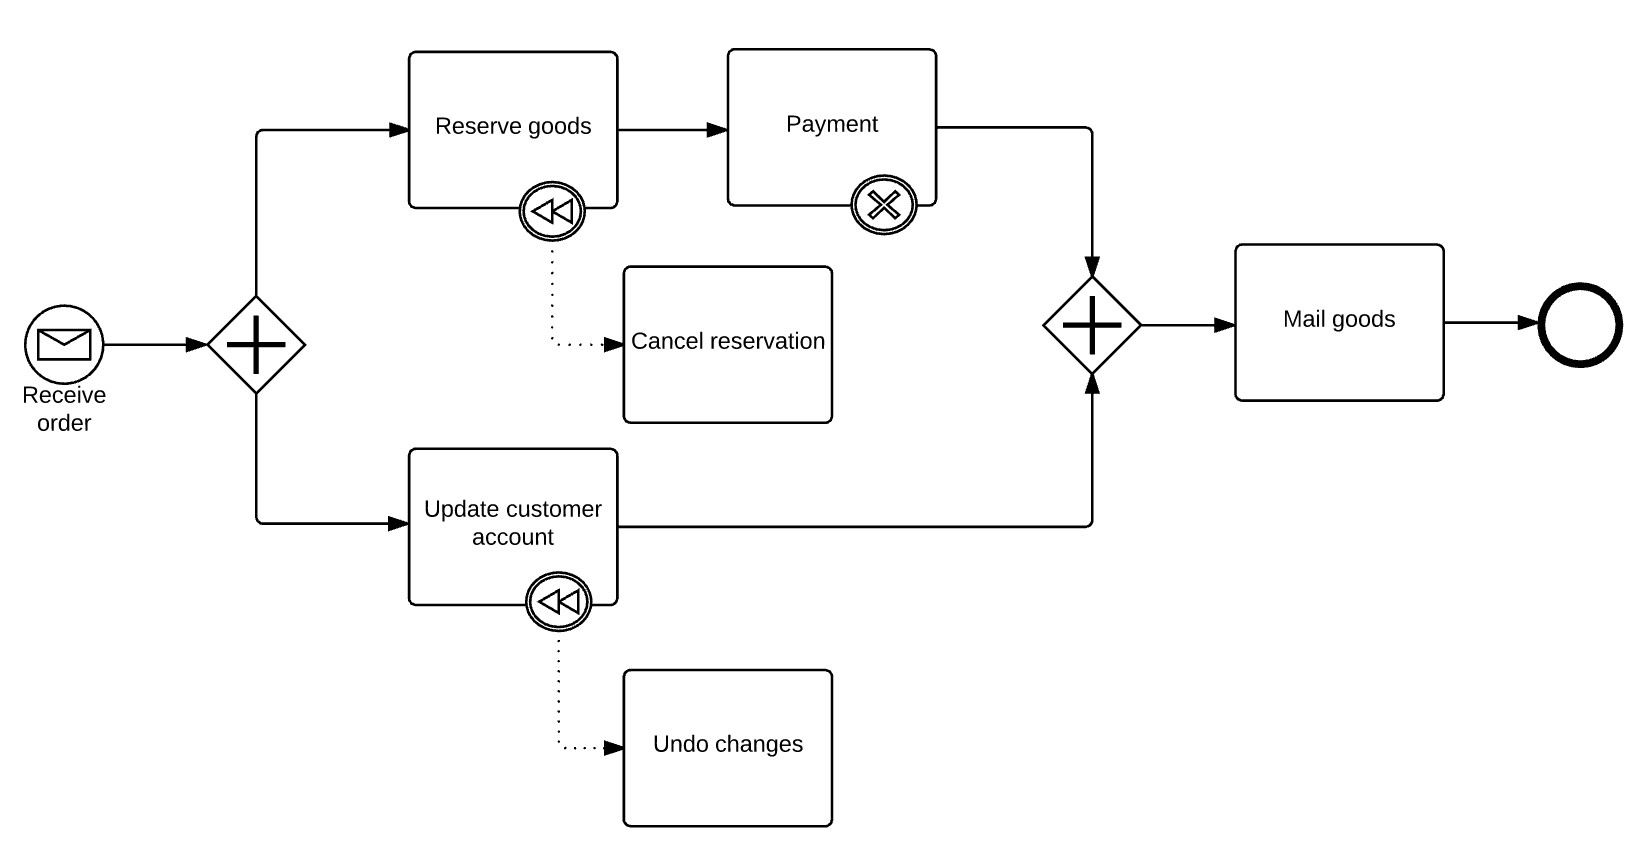
\includegraphics[width=1.75\textwidth]{img/bpmncase1.png}
    }
  \end{center}
  \caption{An example of a sales process modeled in BPMN}
  \label{fig:bpmncase1}
\end{figure}

Figure \ref{fig:reo1case1} shows a Reo network that simulates this process. Here, we use alphabet characters to refer to nodes (e.g. B, C) and channels (e.g. BC, BD). To address a node end or a channel end, we 
%Our formalism deals with data flow in the level of primitive ends. We
append a number to the name of an end, unless it is the only end (e.g. it is a boundary end). %(node or channel end) to refer to distinguish each end. 
For instance, the end $BC_{2}$, which is the source end of the channel $BC$ connects to the end $B_2$ on the node $B$. %For instance, in the example, the end $BC_{2}$  that belongs to \emph{FIFO}$_1$ (BC) that belongs to the    
In \cite{behnaz}, the authors defined a procedure to map BPMN models to Reo networks. % has been presented . %A proof of concept implementations of the BPMN to Reo transformation and the presented constraint-based framework can be found in \cite{mygithubatlb2r} and \cite{mygithubcoloring}, respectively.  %However, a brief explanation follows: 

%\begin{figure}[!h]
  %\begin{center}
  %\scalebox{.6}{
  %\includegraphics[width=0.8\textwidth]{images/newfinal.png}%{screenshot}
 % }
%  \end{center}
  %
%\end{figure}

\tikzstyle{every state}=[node distance=3.0cm]
\begin{figure}[!h]
\centering
\scalebox{.99}{
  \tikz{    
  %\newcommand{\mypsync}{
   % \begin{tikzpicture}[>=stealth]
    %   \filldraw [black] (0,0) circle (1pt) (1,0) circle (1pt);
     %  \draw [->,thick] (0,0) -- (1,0);
      % \node[] at (0.5,0) {$!$};
   % \end{tikzpicture}  
%}
%%%%%%%%%%%%%%%%%%
    \begin{scope}[shift={(0,6.3)}]
    \node [label=left:$W_1$] at (2.7, 5) (BW1) {};
    \node [point, label=left:$W_2$] at (.7, 2) (BR1) {};
    \node [point, label=left:$R_1$] at (.7, 0.5) (BR2) {};
    \node [label=right:$R_2$] at (6.3, 5) (RR2) {};
    \node [label=right:$R_3$] at (7.8, 2) (RR3) {};

    
    \node[point,label=below:$N$] at (1, 0.5) (BN2){};
        \node[point,label=above:$1$] at (1.3, 0.5) (EN1){};
        \node[point,label=above:$2$] at (.7, 0.5) (EN2){};

                        \draw [-, thin] (EN1) -- (BN2);
                        \draw [-, thin] (EN2) -- (BN2);


    \node[point,label=below:$M$] at (2.5, 0.5) (M){};
    \node[point,label=above:$2$] at (2.2, 0.5) (EM1){};
    \node[point,label=above:$1$] at (2.8, 0.5) (EM2){};
    
                            \draw [-, thin] (EM1) -- (M);
                            \draw [-, thin] (EM2) -- (M);


    \node[point,label=below:$C$] at (3.5, 3) (BC1){};
    \node[point,label=above:$1$] at (3.2, 3) (EC1){};
    \node[point,label=above:$2$] at (3.8, 3) (EC2){};
    
                        \draw [-, thin] (EC1) -- (BC1);
                        \draw [-, thin] (EC2) -- (BC1);

    
    \node[point,label=below:$E$] at (5, 3) (BE1){};
    \node[point,label=above:$1$] at (4.7, 3) (EE1){};
    \node[point,label=right:$2$] at (5, 3.3) (EE2){};
    \node[point,label=right:$3$] at (5.3, 3) (EE3){};
    
                    \draw [-, thin] (EE1) -- (BE1);
                    \draw [-, thin] (EE2) -- (BE1);
                    \draw [-, thin] (EE3) -- (BE1);

	\node[point,label=below:$D$] at (3.5, 1) (D1){};
    \node[point,label=above:$1$] at (3.2, 1) (ED1){};
	\node[point,label=above:$2$] at (3.8, 1) (ED2){};
    
                \draw [-, thin] (ED1) -- (D1);
                \draw [-, thin] (ED2) -- (D1);

    
    \node[point,label=below:$F$] at (5, 1) (F1){};
    \node[point,label=above:$2$] at (5, 1.3) (EF1){};
    \node[point,label=below:$1$] at (4.7, 1) (EF2){};
    \node[point,label=below:$3$] at (5.3, 1) (EF3){};
    
            \draw [-, thin] (EF1) -- (F1);
            \draw [-, thin] (EF2) -- (F1);
            \draw [-, thin] (EF3) -- (F1);

	\node[point,label=left:$G$] at (6, 2) (G1){};
    \node[point,label=below right:$2$] at (5.8, 1.8) (EG1){};
	\node[point,label=above right:$1$] at (5.8, 2.2) (EG2){};
	\node[point,label=above:$3$] at (6.3, 2) (EG3){};
    
        \draw [-, thin] (EG1) -- (G1);
        \draw [-, thin] (EG2) -- (G1);
        \draw [-, thin] (EG3) -- (G1);


    \node[point,label=below:$H$] at (7.5, 2) (H1){};
    \node[point,label=above:$1$] at (7.2, 2) (EH1){};
    \node[point,label=above:$2$] at (7.8, 2) (EH2){};

    \draw [-, thin] (EH1) -- (H1);
    \draw [-, thin] (EH2) -- (H1);


    \node[point,label=above:$J$] at (4.5, 5) (J1){};

    \node[point,label=above:$1$] at (4.2, 5) (EJ1){};
    \node[point,label=above:$2$] at (4.8, 5) (EJ2){};
    \node[point,label=left:$3$] at (4.2, 4.7) (EJ3){};
    \node[point,label=left:$4$] at (4.8, 4.7) (EJ4){};
   % \node[rotate=-90] at (5, 4) (prio) {!};
    
    \draw [-, thin] (EJ1) -- (J1);
    \draw [-, thin] (EJ2) -- (J1);
    \draw [-, thin] (EJ3) -- (J1);
    \draw [-, thin] (EJ4) -- (J1);
    
    \node[point,label=above:$I$] at (3, 5) (I1){};
        \node[point,label=above:$2$] at (3.3, 5) (EI1){};
                \node[point,label=above:$1$] at (2.7, 5) (EI2){};
        \draw [-, thin] (EI2) -- (I1);

    \node[point,label=above:$K$] at (6, 5) (K1){};
    \node[point,label=above:$1$] at (5.7, 5) (EK1){};
    \node[point,label=above:$2$] at (6.3, 5) (EK2){};
    
        \draw [-, thin] (EK1) -- (K1);
        \draw [-, thin] (EK2) -- (K1);


    \node[point,label=right:$B$] at (2.5, 2) (B1){};
    \node[point,label=above left:$1$] at (2.2, 2) (EB1){};
    \node[point,label=left:$3$] at (2.5, 1.7) (EB2){};
    \node[point,label=left:$2$] at (2.5, 2.3) (EB3){};
    
            \draw [-, thin] (EB1) -- (B1);
            \draw [-, thin] (EB2) -- (B1);
            \draw [-, thin] (EB3) -- (B1);

    \node[point,label=below:$A$] at (1, 2) (A1){};
    \node[point,label=above:$1$] at (.7, 2) (EA1){};
    \node[point,label=above:$2$] at (1.3, 2) (EA2){};
    
                \draw [-, thin] (EA1) -- (A1);
                \draw [-, thin] (EA2) -- (A1);

    \node[point,label=left:$L$] at (3.8, 2) (L){};
    \node[point,label=right:$1$] at (3.8, 2.3) (EL1){};
    \node[point,label=right:$3$] at (4.2, 2) (EL2){};
    \node[point,label=right:$2$] at (3.8, 1.7) (EL3){};
    
                    \draw [-, thin] (EL1) -- (L);
                    \draw [-, thin] (EL2) -- (L);
                    \draw [-, thin] (EL3) -- (L);

    \draw[psync]  (EE2) to node {} (EJ4);%priority
	\draw[lossysync]  (EJ3) to node {} (EL1);
    \draw[syncdrain]  (EL2) to node {} (EF1);
    \draw[sync]  (EL3) to node {} (EM2);
	\draw[sync]  (I1) to node {} (EJ1);
	\draw[sync]  (EA2) to node {} (EB1);
	\draw[smallfifo]  (EM1) to node {} (EN1);
    \draw[smallfifo]  (EC2) to node {} (EE1);
    \draw[smallfifo]  (ED2) to node {} (EF2);
    \draw[smallfifo]  (EG3) to node {} (EH1);
    \draw[smallfifo]  (EJ2) to node {} (EK1);
    %%%
    \draw[smallfifo]  (EE3) to node {} (EG2);
    \draw[smallfifo]  (EF3) to node {} (EG1);
    \draw[smallfifo]  (EB3) to node {} (EC1);
    \draw[smallfifo]  (EB2) to node {} (ED1);

    \draw [-, thick, fill=white] (BN2) circle (3pt);%n
    \draw [-, thick, fill=white] (M) circle (3pt);%m
    \draw [-, thick, fill=white] (3.8, 2) circle (3pt);%l
    \draw [-, thick, fill=white] (A1) circle (3pt);%a
     \draw [-, thick, fill=white] (BC1) circle (3pt);%c
    \draw [-, thick, fill=white] (H1) circle (3pt);%h
    \draw [-, thick, fill=white] (2.5, 2) circle (3pt);%b
    \draw [-, thick, fill=white] (G1) circle (3pt);%g
    \draw [-, thick, fill=white] (D1) circle (3pt);%d
    \draw [-, thick, fill=white] (BE1) circle (3pt);%e
    \draw [-, thick, fill=white] (F1) circle (3pt);%f
    \draw [-, thick, fill=white] (BE1) circle (3pt);%e
    \draw [-, thick, fill=white] (J1) circle (3pt);%j
    \draw [-, thick, fill=white] (K1) circle (3pt);%k
    \draw [-, thick, fill=white] (I1) circle (3pt);%i
    %node decorations
    \node[] at (G1) {\textbf{$+$}};
    \node[] at (J1) {\textbf{$+$}};
    \node[] at (F1) {\textbf{$\times$}};
   	\node[] at (BE1) {\textbf{$\times$}};
\end{scope}
}
}%scalebox
\caption{The process of a sample on-line shop modeled in Reo}
    \label{fig:reo1case1}
\end{figure}

The process starts by reading a token from the \emph{writer} $W_2$, which resembles receiving an order. Though a Reo network can be used for modeling infinite data flow, in the BPMN standard, when a \emph{start} event is triggered, 
a new instance of the process is instantiated. Therefore, the Reo network is designed to handle only one request. The end $A_1$ reads a token from the writer \emph{W$_2$} and duplicates it into the \emph{BC} and \emph{BD} \emph{FIFO$_1$} channels.
 The token continues to the \emph{CE} \emph{FIFO$_1$} channel. If the payment succeeds, the token enters the \emph{EG} \emph{FIFO$_1$} channel waiting for a token from the other input of the \emph{merge} node \emph{G} to enter the \emph{GH} \emph{FIFO$_1$} channel and finally to be consumed by the \emph{reader} $R_3$.
 
If the payment fails, performed actions need to be compensated. A token from the writer $W_1$ indicates a payment failure, so the process needs to be canceled. So, the token leaving the \emph{CE} \emph{FIFO$_1$} channel goes through the \emph{EJ} \emph{prioritySync} channel. The \emph{replicate} node \emph{J} duplicates the token to the \emph{JK} \emph{FIFO$_1$} and the \emph{JL lossySync} channel. 
%Note that the \emph{cancel} event attached to the \emph{payment} process is triggered under relevant conditions. For simplicity, here we have abstracted away from this conditions. %We simulate these alternating flows using the priority agnostic \emph{merger} \emph{E}, where it chooses one of its outgoing edges non-deterministically.
 The \emph{reader} $R_2$ consumes the token from the \emph{JK} \emph{FIFO$_1$} channel, while the token from the \emph{JL lossySync} channel moves forward to the \emph{MN FIFO$_1$} channel. % representing the \emph{undo change} task.

The token from the \emph{BD} \emph{FIFO$_1$} channel goes through the \emph{DF FIFO$_1$} channel for a possible  compensation. The token from the \emph{DF FIFO$_1$} channel may either go to the \emph{join} node \emph{G} to join the flow of a successful payment, or to be consumed by the \emph{LF syncDrain}. In the latter case, it goes to the \emph{MN} \emph{FIFO$_1$} channel. Then, the process ends by a read action of the \emph{reader} $R_1$.

%For clarity, we have labeled each node and channel ends. % in Figure \ref{fig:albelednetwork1}.
We compute the behavior of the given Reo network using our constraint-based framework. % resulting in the Reo LTS of 
%Figure/Listing ?? represents a constraint, which encodes the behavior of the network. ??? provides the solutions for the constraint of ???. Using our mapping ???, the ??? behavior of the network 
 %Figure \ref{fig:case1behavior}.
The steps for obtaining the RLTS are as follows: First, we form the RCSP of the network by traversing through its primitives. Then, we solve the obtained RCSP and extract transitions from obtained solutions.% ,  to a transition (along with its source and target states)   as described in Algorithm \ref{alg:solvercsp}.
 
To show how priority can affect the behavior of our example, we first investigate the behavior of the network in absence of priority, wherein the normal flow of the process can continue even in case of a payment failure. This is because the \emph{router} nodes \emph{E} chooses one of its outgoing flows in a non-deterministic fashion. %Therefore, it is possible to have the transition $t_4$ from the state $s_3$ to the state $s_4$, even though the \emph{writer} $W_1$ is ready to communicate. % ($W_1$ is not in the $N_2$ set of $t_4$). %For the sake of brevity, here we omit some nodes (which are either obvious from context or not important for our example) in $N_1, N_2$, marked by '...'.

We would like to check if for all transitions $t$, which belong to the RLTS of the network, the following holds: $\{CE,$ $ DF\} \subseteq source(t) \wedge E_1 \in flow(t) \wedge W_1 \notin reason-giving(t) \Rightarrow W_1 \in target(t)$. To violate this property, it is enough to find a transition from a state wherein both $CE$ and $DF$ \emph{FIFO}$_1$ channels are full, there is flow on end $E_1$, $W_1$ is ready to communicate, but $W_1$ does not have flow.

\emph{Abstraction}: 
For checking this assertion, we abstract from the ends without flow on transitions with the same source ($q$), target ($p$), ends with flow ($N_1$), but different ends without flow ($N_2$) by replacing them with $\longtransition{q}{N_1, {N'}_2}{p}$, where ${N'}_2=\{W_1\}$ if $W_1 \in N_2$, otherwise ${N'}_2=\{\}$. This abstraction reduces the number of transitions in the RLTS without affecting the result of the verification for the given assertion. We can take this one step further and remove the information about ends without flow from all the states except the state wherein $CE$ and $DF$ \emph{FIFO}$_1$ channels are full.

Figure \ref{fig:case1behaviorwoprority} shows the abstract (with respect to the given assertion) RLTS of the network of Figure \ref{fig:reo1case1} in absence of priority, where the transition $t_4$ violates the assertion. Here, we use short labels (e.g. $t_4$) on transitions and states. The original labels are represented in Table \ref{tbl:labelscase1behaviorwoprority}. In addition, the ends with a similar name are grouped e.g. $B_{1,2,3}$ (referring to ends $B_1$, $B_2$, and $B3$). This is only a presentation modification to save space. We show that the transition $t_4$ can not exist when the priority is considered in the model.

$$0: \mathring{CE} \wedge \mathring{DF} \wedge \tilde{E}_1 \wedge \neg {W_1}^\triangleright \wedge \neg \tilde{W}_1 \ (the\ assertion)$$

$$1:\frac{\Psi_{PrioritySync}(EJ_{2,4}) }{EF_2^{!^\bullet} } $$ %($ef_2$ has priority)

$$2:\frac{1\ \& \text{join of } EJ_2 \& E_2}{E_2^{!^\bullet}}$$ %($e_2$ has priority)

$$3:\frac{2; \Psi_{router}(E_{1,2,3}) }{\tilde{E_1} \wedge \neg 
\tilde{E_2} \Rightarrow {E_2}^\triangleright} \ $$
%\text{Join axiom for} ef_2 \text{ and } e_2}

$$4:\frac{3\ \&\ \text{coloring}\ \&\ \text{join}}{ {E_2}^\triangleright \Rightarrow {W_1}^\triangleright}$$ 

$$5:\frac{2\ \&\ 4\ \text{coloring}\ \&\ \text{join}}{\neg \tilde{W}_1\Rightarrow {W_1}^\triangleright} $$

$$6:\frac{0 \& 5}{\bot}$$

%
\begin{center}
\begin{figure}[t]
%\sub figure[\scriptsize{CA-based semantic model}]{
     \tikz[scale = 1]{
          \node[circle, draw] at (0, 4) (p) {$s_1$};
          %\node at (1,7.8)(lp) {state:1};
          \node[circle, draw] at (1.5, 4) (q) {$s_2$};
          %\node at (4,7.8)(lq) {state:2};
          \node[circle, draw] at (3, 4) (r) {$s_3$};
         % \node at (8,7.95)(lr) {state:3};
          \node[circle, draw] at (4.5, 4) (s) {$s_4$};    
     %     \node at (12,7.95)(ls) {state:4};
          \node[circle, draw] at (6, 4) (t) {$s_6$}; 
                  %  \node at (12,4.55)(lt) {state:6};
          \node[circle, draw] at (3, 2.5) (u) {$s_5$};
             %       \node at (4,5.05)(lu) {state:5};
          \node[circle, draw] at (1, 2) (x) {$s_7$};
         %       \node at (1,3.15)(lx) {state:7};
          \node[circle, draw] at (5, 2) (z) {$s_8$};
             %    \node at (7,3.15)(lz) {state:8};
         %
          \node[circle, draw] at (3, 1.5) (y) {$s_9$};
         % \node at (4,2.25)(ly) {state:9};
          \node[circle, draw] at (7.5, 4) (a) {$s_{10}$};
       %   \node at (12,2.14)(la) {state:10};
%\node at (.5, .2) (prio) {};
     % \node[text width=1cm, circle, draw] at (2+6, 6) (u2) {$r_1:1,$ \\ $r_2:1,$ \\ $r_3:1$ \\ $JK,FG$};
     %\node[text width=1cm, circle, draw] at (0+5.5, 4) (x2) {$r_2:1,$ \\ $r_3:1$ \\ $JK,FG$};
     %\node[text width=1cm, circle, draw] at (4+6.25, 4) (z2) {$r_1:1,$ \\ $r_3:1,$\\ $MN,FG$};
   %       \node[text width=1cm, circle, draw] at (2+6, 3.5) (y2) {$r_1:1$\\$r_3:1$\\$FG$};
      %p to q
          \path[transition]
          (p) edge [bend left=0] node[above] { $t_1$ } (q)
          (q) edge [bend left=0] node[above] { $t_2$ } (r)
          (r) edge [bend left=0] node[left] { $t_3$ } (u)
  %r to u2
%            (r) edge [bend left=0] node[above] { $N_1$:\{$W_1,J_{1,2,3,4},E_{1,2},L_{1,2,3},F_{1,2},M_{1,2},...$\},$N_2:\{F_3,FG_2,EG_1,E_3,G_3,...\}$ } (u2)
          (r) edge [bend right=0] node[below] {$t_{10}$} (s)
          (u) edge [bend left=0] node[above] {$t_5$} (x)
          (u) edge [bend left=0] node[left] { $t_6$ } (y)
          (u) edge [bend left=0] node[above] { $t_7$ } (z)       
          (x) edge [bend left=0] node[below] { $t_8$ } (y)
          (z) edge [bend left=0] node[below] { $t_9$ } (y)
 %         (r) edge [bend left=-30] node[below] { \{$E_1$, $E_2$, $F_1$, $F_2$, $F_3$, $L_1$, $L_3$\} } (v)
 %         (v) edge [bend left=-30] node[left] { \{$G$\} } (w)
          (r) edge [bend left=40] node[above] { $t_{4}$ } (s)
          (s) edge [bend left=0] node[above] { $t_{11}$ } (t)
          (t) edge [bend right=0] node[above] { $t_{12}$ } (a);
       }
\caption[Ignoring priorities in Figure \ref{fig:reo1case1}]{The RLTS corresponding to Reo network of Figure \ref{fig:reo1case1} with no priority channel}
\label{fig:case1behaviorwoprority}
\end{figure}
\end{center}
\begin{table}[t]
\caption[Priority data of Figure \ref{fig:case1behaviorwoprority}]{The transition labels and prioritized ends (P) of the RLTS of Figure \ref{fig:case1behaviorwoprority}
}
\begin{tabular}{|c|l|}
\hline
$s_1$ & $\langle \rangle$\\
$s_2$ & $\langle BC, BD \rangle$\\
$s_3$ & $\langle CE, DF \rangle$\\
$s_4$ & $\langle EG, FG \rangle$\\
$s_5$ & $\langle MN, JK \rangle$\\
$s_6$ & $\langle GH \rangle$\\
$s_7$ & $\langle JK \rangle$\\
$s_8$ & $\langle MN \rangle$\\
$s_9$ & $\langle \rangle $\\
$s_{10}$ & $\langle \rangle$\\
$t_1$ & $N_1:\{W_2,A_{1,2},B_{1,2,3},AB_{1,2},BC_{2},BD_{3}\},N_2:\{\}$\\
$t_2$ & $N_1:\{BC_{1},BD_{1},C_{1,2},D_{1,2},CE_{2},DF_{2}\},N_2:\{\}$\\
$t_3$ & $N_1:\{W_1,CE_{2},DF_{3},IJ_{2,3},I_{1,2},J_{1,2,3,4},JK_{2},
JL_{1,3},$\\
&$L_{1,2,3},LF_{2,3},LM_{1,2},F_{1,2},M_{1,2},MN_{2}\},N_2:\{\}$\\
$t_4$ & $N_1:\{EG_3,FG_3,E_{1,3},F_{1,3},CE_1,DF_1\},$\\
&$N_2:\{W_1\}$\\
$t_5$&$N_1:\{R_1,N_{1,2},MN_1\},N_2:\{\}$\\
$t_6$&$N_1:\{R_{1,2},N_{1,2},MN_1,K_{1,2},JK_1\},N_2:\{\}$\\
$t_7$ & $N_1:\{R_2,K_{1,2},JK_1\},N_2:\{\}$\\
$t_8$ & $N_1:\{R_2,K_{1,2},JK_1\},N_2:\{\}$\\
$t_9$ & $N_1:\{R_1,N_{1,2},MN_1\},N_2:\{\}$\\
$t_{10}$ & $N_1:\{EG_3,FG_3,E_{1,3},F_{1,3},CE_1,DF_1\},$\\
&$N_2:\{W_1\}$\\
$t_{11}$ & $N_1:\{EG_{1},FG_{2},G_{1,2,3},GH_{3}\},N_2:\{\}$\\
$t_{12}$ & $N_1:\{R_3,H_{1,2},GH_1\},N_2:\{\}$\\
P & $\{W_1, I_{1,2}, J_{1,2,3,4},
JK_{2}, EJ_{2,4}, E_{1,2}, JL_{1,3}, L_{1,2,3},$ \\ 
&$LF_{2,3}, F_{2,3}, LM_{1,2}, M_{1,2}, MN_{2}\}$\\
\hline
\end{tabular}
\label{tbl:labelscase1behaviorwoprority}
\end{table}
%\input{computation}

\section{Related work}
\label{sec:relatedWork}
%Apart from pure scripting languages, an important class of workflow languages is graph-based languages. While the functional and behavioral aspects are represented by directed graphs, the informational and operational aspects require additional textual specifications. At the foundation level, textual annotations of concurrent processes can be based on process algebras with priority~\cite{Cleaveland:2007:PAP:1282576.1282847}. 
 %Our Reo-based approach models a process by directed graphs, which is easier to understand than textual notations. Moreover, Reo-based models are rigorous enough to enable automated analysis.
Several works, e.g., \cite{Furicht:2002:CAF:564092.564117,petriprio,Bause1997} use priorities to model 
scheduling policies. Many workflow languages rely on Petri nets~\cite{Aalst02workflowpatterns,vanderAalst:2005:YYW:1187495.1187496}.
Priority flow in Petri net-based process models is managed with the help of inhibitor arcs and transition priorities~\cite{Padberg2015}. Inhibitor arcs allow a transition to fire only if the adjacent place is empty. \emph{Prioritized Petri nets} 
\cite{Balbo2001} introduce a partial order on transitions. Given a set of enabled transitions, the transitions with higher priority fire before the transitions with lower priority. Others, e.g.,  \cite{DBLP:journals/fuin/LomazovaP16,VALERO2012290} use a partial order on transitions to model priority. Our earlier approach in modeling priority using binary variables supports a limited form of priority compared to the mentioned Petri nets approaches. However, the proposed extension bridges this gap by defining priorities as non-zero natural numbers. An advantage of our model is its compositionality. Compared to the aforementioned methods, Reo fits in the realm of component-based or service-oriented architecture in a compositional way. Reo is an extensible language, where new behavioral aspects can be added. An effort to express the behavior of Reo networks via constraints is reported in \cite{ClarkeProenca10}. It demonstrates the efficiency of the constraint-based approach. It models synchronization and data flow constraints, but no priority flow was considered. In \cite{behconstraint}, a framework is presented to encode semantics of Reo networks as CSP with predicates in the form of binary propositions and numerical constraints. An advantage of this method is handling data constraints symbolically and, hence, mitigating the state explosion problem of automata models. We extended this framework to handle priority constraints, taking a step forward toward implementing a tool-set that covers all behavioral aspects of Reo. Among the formal semantics of Reo, connector coloring comes with a limited notion of priority based on the context information. The context information affects otherwise non-deterministic data-flow choices. In \cite{KappeAT16}, an automata-based semantics is proposed, which associates a preference for each transitions. A transition of lower preference is fired iff no more preferred transition can occur.

\section{Conclusions and future work}
\label{sec:conclusionsprio}
In this chapter, we addressed the problem of priority flow modelling using the Reo coordination language.
We extended the unified constraint-based semantics of Reo with binary and numeric priority constraints. Furthermore, we showed correctness of our approach for the binary case. %and evaluated the performance of the algorithm for  solving the RCSP to derive the semantics of a Reo network given the behavior of its constituent??? elements.
We also illustrated the use of our framework for modeling business processes with priority flow.
%In this chapter, we have incorporated priority into Reo networks to support modeling of business processes with priority. We have extended the unified constraint-based semantic model of Reo with priority. We have presented our solution in a step-wise manner. First, we have modeled binary priorities and after showing correctness of our approach and evaluating its performance, we have extended it into numeric priority. 

As part of our ongoing work, we are using this framework to encode other aspects of the semantics of Reo, specifically, timed behavior. A promising area for future work is to use our framework for constraint-based model checking of Reo networks with priority. 
%Finally, we will create a library of useful coordination patterns, including those with priority flow.
